\chapter{Contribution} \label{chap:contribution} % 30-40 pages

In this chapter, the use case and its challenges are presented, before we go into detail of how the GAN has to be adapted to allow forecasting of future frames in video. We also provide a step by step analysis of our modifications to the GAN that we used as the baseline architecture for our final model. Afterwards, we present our modifications to IFTM and how our GAN model is integrated into the framework. Then, our large-scale evaluation data set is presented and formally analyzed for some of its properties. The chapter closes with a summary of how all of this is combined into our anomaly detection system. An implementation of the different GANs, IFTM, and the rest of our analysis framework is available online\footnote{\url{https://github.com/fshofmann/video-anomaly-detection}}.



% Use Case CCTV Anomaly Detection
\section{CCTV Use Case} \label{sec:use_case}

As we described the challenges of video anomaly detection (VAD) in CCTV systems in Section \ref{sec:cctv} and explained why this kind of analysis requires the automated processing of a high amount of video data that is produced continuously, we decided to evaluate our VAD approach for the following CCTV related use case: A CCTV IP camera\footnote{\href{https://www.upcam.de/en/ip-cameras/upcam-cyclone-indoor/upcam-cyclone-hd-eco/176/upcam-cyclone-hd-eco-black-all-in-one-surveillance-camera}{upCam Cyclone HD eco}} for interior surveillance is stationed in a home office to monitor the behavior and changes of the person working there. This location was chosen by us both due to the current ongoing pandemic  and any privacy concerns that may arise when recording third parties without their knowledge: According to the German Federal Data Protection Act the recording of such is only allowed in reason if only private property is monitored and the people recorded on video have explicitly given their consent \cite{brd2017fdpa}. Furthermore the proportionality has to be considered as well. To avoid any legal troubles, only the person working in the home office and the people living in the same household were captured by the camera.

The camera's position, viewing angle, direction, and field of view is overall static. This results in a more or less static scene as shown in Figure \ref{fig:room}: In the middle, one can see the desk and the office chair, surrounded by a shelf from the left side and a lowboard from the right. A bed is also present in the room. The person working there usually sits at the desk, moves in and out of the room and also sleeps in the mentioned bed during the night. Writing utensils and papers are sometimes stored on the lowboard and desk next to them. Occasionally other people enter the room, but mostly the working person is the only one present. Finally in the top right, a timestamp is attached to every video frame. 

\begin{figure}
	\centering
	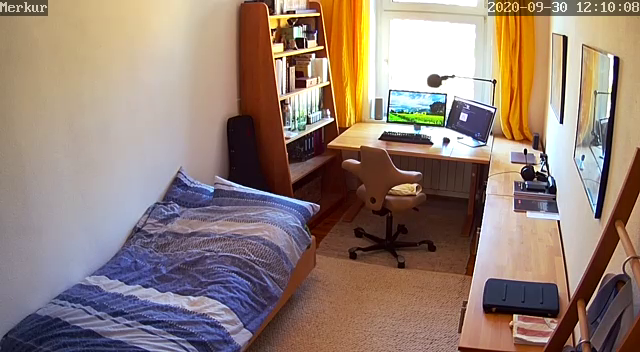
\includegraphics[width=0.9\textwidth]{graphics/cctv/room.png}
  \caption[View of the monitored room.]{Static view of the (empty) monitored room.}
  \label{fig:room}
\end{figure}

The IP camera's video feed is streamed via RTSP to a network attached storage and stored on a 30 day ring-buffer. The video stream is segmented  into one hour-long videos, with a resolution of $640 \times 352$ and a varying FPS of 2.5--5. The variance is explained by the (grayscale) night vision mode, that has fewer frames per second than the colored day vision. This results in the generation of around one gigabyte of unfiltered and unprocessed video data per day. We will expand on the properties and the preprocessing of the collected video data in Section \ref{sec:dataset}.\\

When using an anomaly detection system (ADS) to identify anomalous frames in that video stream, one has to learn and identify the different normal object patterns that people and objects in that video feed have. As explained in Section \ref{subsec:anomaly_types}, understanding the context in which an event is happening is often as equally important as the event itself. And to identify collective anomalies in the video, one has to analyze frames in context with their predecessors. But, due to the varying frame rate, it is difficult for a model to understand how much time truly has passed --- it could extract that information from the timestamp, but this would be costly. Instead, the video frame rate has to be stabilized. In addition, the resolution is impractical for some kind of models, which requires a specific constrained input format. Since there are no labels attached to any frames of the video data available, training of the ADS must be done in an unsupervised mode. This means one has to assume that the raw video data is mostly considered normal and that the underlying model of the ADS will not be corrupted by any potential anomalies found during training. Ideally, these anomalous properties and features are forgotten and cast away by a model that should only represent normal features. 

Finally during the detection phase after the training of the model is completed, we only want to process frames of the (theoretically infinite) video stream once: The detection method is required to label each frame of the video, using only the preceding frames and its knowledge of the training data. This creates the need of several modifications to the underlying model which IFTM uses to represent the normal state and how the data has to be processed --- this will be described in the following section.



% C-GAN for Video Prediction
\section{C-GAN for Video Forecasting} \label{sec:cvgan}

In this section we describe and discuss our model for video generation forecasting. The model's characteristics are based on the generative adversarial network for video (VGAN) by Vondrick et al. \cite{vondrick2016generating}. During every modification step, we first present how the original architecture was designed, for what it was intended, and why and how we adapted it. First, the general VGAN architecture is modified, before we continue with its conditional version (C-VGAN)\nomenclature{C-VGAN}{Conditional generative adversarial network for video}. Finally we will present our proposed modification to C-VGAN to accept spatio-temporal data, i.e. multiple video frames. Each of the adapted models from the intermediate steps is fully functioning on its own, although not fully evaluated, because it is not of interest to the use case.


\subsection{VGAN} \label{subsec:vgan_mod}

Building on the successes of GANs and the constrained DCGAN architecture, that leverages large amounts of unlabeled images to generate realistic looking ones, Vondrick et al. propose a novel generative model for video \cite{vondrick2016generating}: Videos with scene dynamics can be dissected into a static background that determines the scene and a dynamic foreground, that is spatio-temporal in nature. Explicitly modeling this property in videos by using a two-stream architecture for the generator, allows the model to learn to untangle these components from each other. This is helpful for example, when the same object dynamics could occur in front of different static scenes. The model learns to generate these two pathways in an unsupervised manner, so when combined following Equation \ref{eq:vgan}, the resulting videos seem real.

\begin{equation} \label{eq:vgan}
G(z)=m(z) \odot f(z) + (1-m(z)) \odot b(z)
\end{equation}

The first of the two streams is spatio-temporal and its output consists of two parts: The actual moving foreground ($f$) and the spatio-temporal mask ($m$) of it. The latter selects or deselects pixels of foreground and background, so moving objects do not overlap parts of the back ground when foreground and background are merged together. To model the temporal information in video, fractionally-strided 3D convolutions are used instead of 2D ones. In addition, the kernel size of the convolutional filter is $4$ along all three dimensions instead of $5$ with a stride of $2$. An exception is the first de-convolutional layer, that instead uses a kernel size of $1$ but a higher stride to upscale the 100-dimensional Gaussian input ($z$) to the fitting size. Convolutional filters range from $512$ for the first layer, to $64$ and then $3$ (RGB color channels) for the last one, halving at every step of the stack. The same structure is used for the background stream ($b$), but because it only has to produce a static image, spatial convolutions without the temporal component are used. Everything besides that matches the foreground stream. As in the DCGAN architecture, the hyperbolic tangent activation function is used for the output layer, except for the mask that uses sigmoid activation. Note, that when aggregating the three tensors $f$, $m$, and $b$ into the final generated video, $b(z)$ has to be transformed into a 3D output to match the other tensors. This is achieved by replicating it across the time dimension, therefore being a static video of $n$ times the same frame. Something similar has to be done to $m(z)$; the mask does not have RGB channels but is only in a range of $[0,1]$ per pixel. So that singleton dimension has to be replicated across the three color channels to match background and foreground output.

For the discriminator, which also follows the DCGAN architecture, the foreground stream is reversed, downsampling a given video to a binary output (real/fake), by repeatedly applying strided spatio-temporal convolutions to the video. Their model produces and discriminates $64 \times 64$ videos that have 32 frames --- little over a second long, and it is used to generate real looking videos from random Gaussian input. As a second alternative application, the discriminator is extended to a K-way classifier to learn action recognition.\\

\begin{figure}
	\centering
	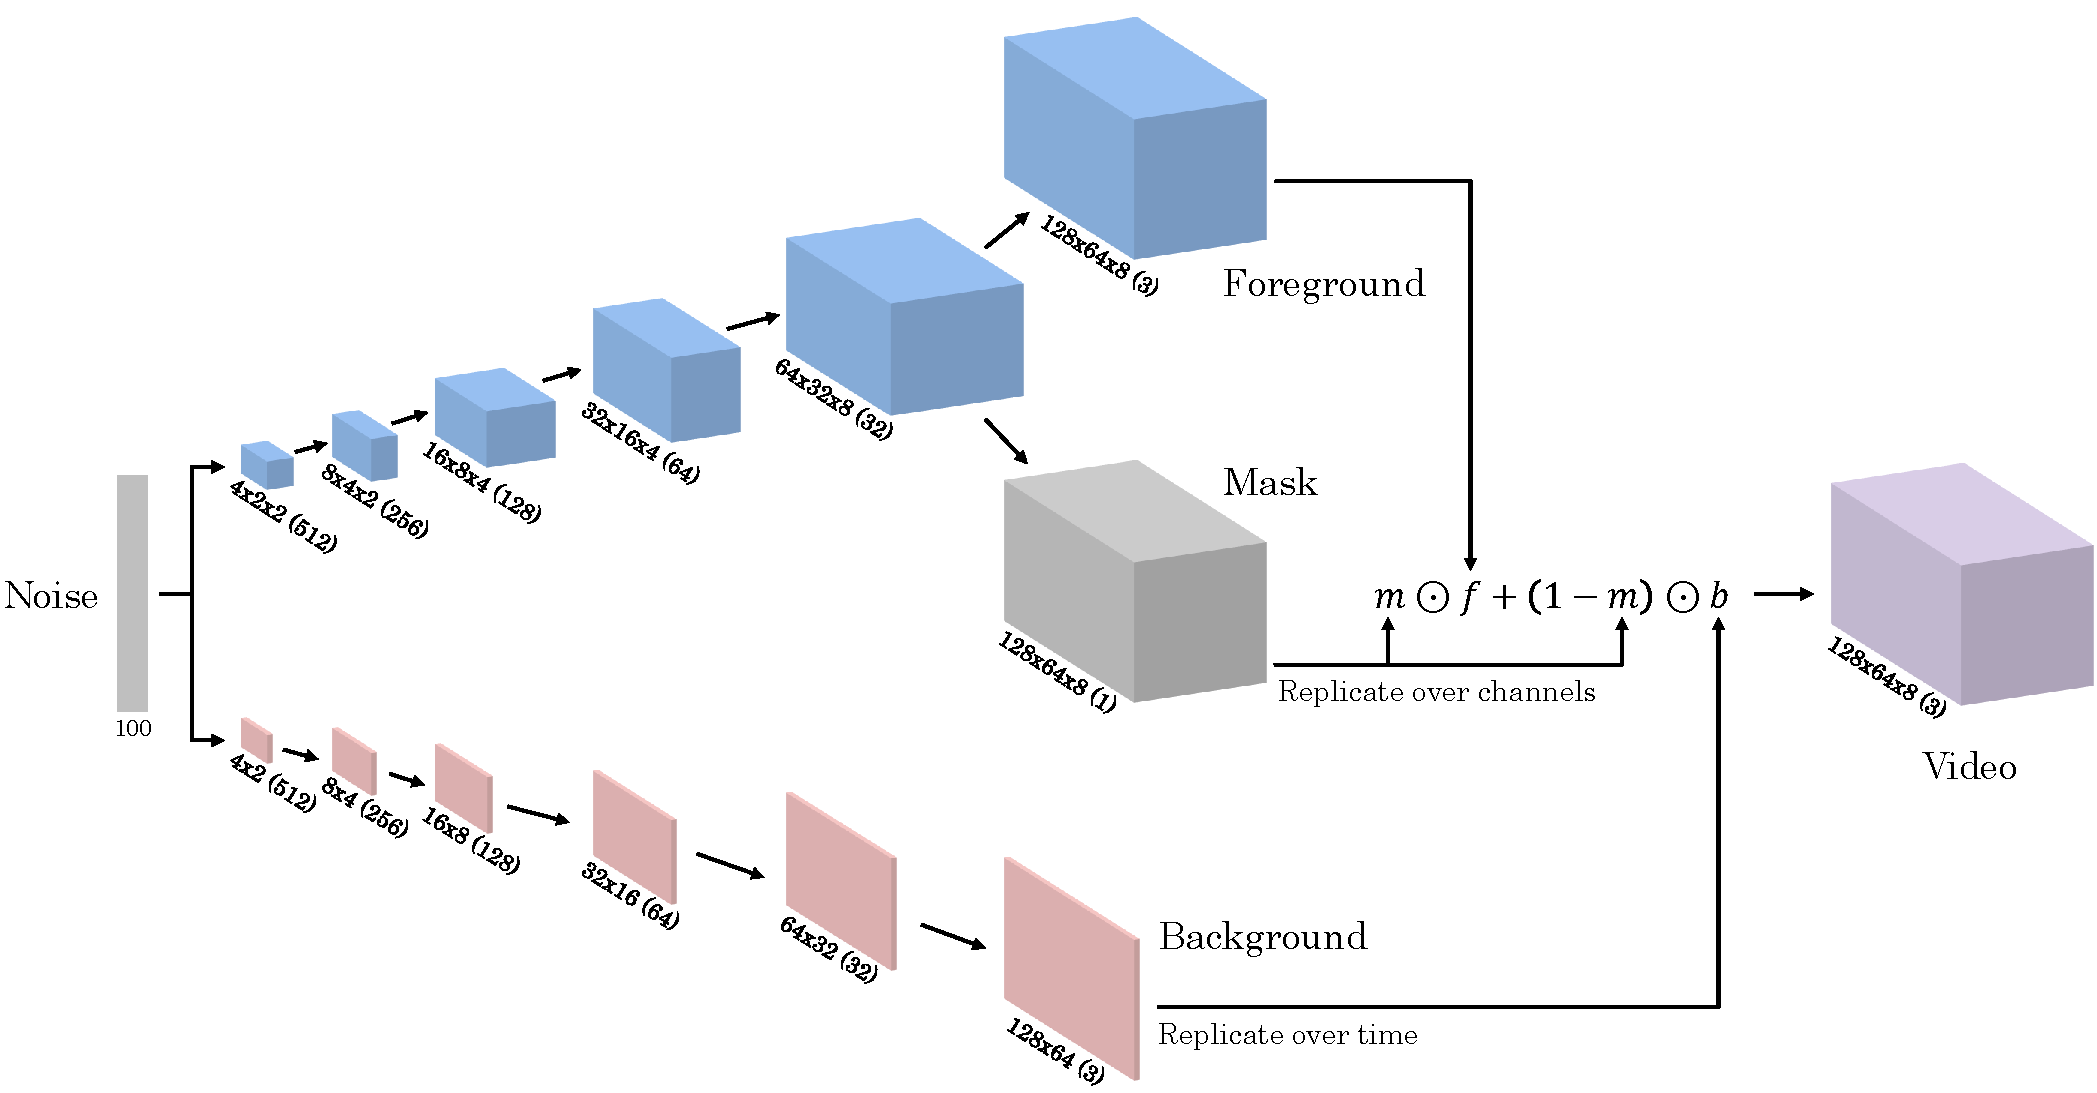
\includegraphics[width=1\textwidth]{graphics/gan/vgan/vgan/vgan_g.pdf}
  \caption[Adapted two-stream video generator network.]{Adapted VGAN generator \cite{vondrick2016generating}. A 100-dimensional random latent vector serves as input for two streams; a dynamic foreground using fractionally-strided spatio-temporal convolutions, and a static background of fractionally-strided spatial convolutions. The number in parentheses is the number of channels for each output, equal to the number of convolutional filters. As the generated video is in RGB, it does have three channels.}
  \label{fig:vgan_g}
\end{figure}

\paragraph{Modifications to VGAN}
For our modifications to VGAN shown in Figure \ref{fig:vgan_g}, the generator had to be adapted to our data first. During preprocessing of our data set as will be explained in Section \ref{subsec:dataset_preprocessing}, the video format was reduced to $128 \times 64$ and the frame rate was stabilized to 5 frames per second. Because this is one sixth the frame rate while the size of a frame has effectively doubled compared to the $64 \times 64$ that VGAN originally produced, it was decided that our generator shall generate videos with a length of $\sim 1.5$ seconds or 8 frames. This still results in less total pixels that need to be generated for a final space-time cuboid (video). On the other hand, the complexity of the background in fact increases, because it doubles in size. Therefore taking the loss and rise in complexity into account, one additional fractionally-strided convolutional layer is added to each stream, while the size of the first convolutional layer is slightly reduced. From $4 \times 4$ in the original VGAN to $4 \times 2$. Furthermore, because 8 frames instead of 32 have to be generated, the stride value along the time axis is only 2 every other convolutional layer. This gives the foreground stream enough space to upsample the frame information. In addition, because according to recent research even-sized convolutional kernels lead to distortions in the output \cite{wu2019convolution}, we change the convolutional layer's kernel size to $3$ across all relevant dimensions for both discriminator and generator. Instead of reshaping the input and feeding it directly into the first convolution, one dense layer for each stream upsamples the latent code to the input size of the first convolutional layer. Therefore, rather than having a kernel size of $1$ and being used as a matrix multiplication to reshape the input \cite{radford2015unsupervised}, the first convolutional layer is already being used for actual convolutional filters with a kernel size of $3$. Finally, weights in the generator network that precede ReLU activations, were not initialized with Gaussian noise ($\mu=0$, $\sigma=0.01$) like in the VGAN or DCGAN architecture. These weights are instead initialized with He normal, a truncated version of a normal distribution with an adaptive standard deviation. With the ReLU function being only positive, this helps with the quality and the convergence speed \cite{he2015delving}. The final convolutional layers' weights in the foreground with hyperbolic tangent and sigmoid activation are on the other hand initialized using the Glorot uniform initializer. The normal distribution used has an adaptive variance, balancing the variance of the input with the output's variance of the layer, which works especially well for these kinds of activations \cite{glorot2010understanding}.

\begin{figure}
	\centering
	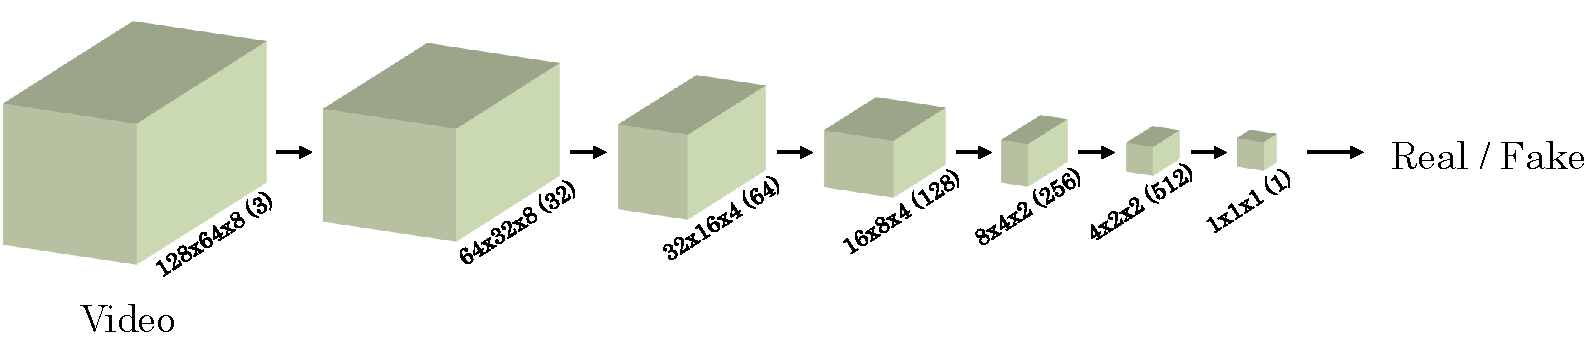
\includegraphics[width=1\textwidth]{graphics/gan/vgan/vgan/vgan_d.pdf}
  \caption[Adapted video discriminator network.]{Adapted VGAN discriminator \cite{vondrick2016generating}; a CNN-based classifier being the reverse of the generator foreground stream. The number in parentheses is the number of channels for each output, equal to the number of convolutional filters.}
  \label{fig:vgan_d}
\end{figure}

Our discriminator, as the original VGAN discriminator model, is the reverse of its counterpart's foreground stream: A spatio-temporal, CNN-based, video classifier with one fully connected neuron for the output. As seen in Figure \ref{fig:vgan_d}, videos are downsampled from $128 \times 64 \times 8$ to $4 \times 2 \times 2$, with the time dimension only halved at every second step in the convolutional stack, as it was done in the generator model.

This model, when trained using unlabeled video data, should only be able to generate (and discriminate) normal video clips of 8 seconds, if the training data is mostly normal. However, it is unfeasible to utilize the generator as a representation of normal behavior, because its outputs are impossible to be compared to the current state of the system: It simply generates random normal looking videos based on random input; this could be videos both during nighttime or daytime even. The discriminator may be of interest because of its ability to distinguish real videos from synthetic ones, but only if one can assume that anomalous observations in video seem ``fake`` to the discriminator. However, this assumption is risky --- the discriminator was trained to learn the properties of the generator network. Thus in the following section, we will look into a modification of VGAN for future frame prediction.


\subsection{C-VGAN} \label{subsec:cvgan_mod}

Vondrick et al. further refined their model to allow generation of a video based on an input frame \cite{vondrick2016generating}: In their published work, they achieved that by attaching a convolutional network as an encoder to the front of the generator network. The encoder mirrors the background stream but is reversed, encoding the $64 \times 64$ frame into latent code ($4 \times 4$, with $512$ channels), that both foreground and background stream then use to upsample from instead of the Gaussian noise. The first convolutional layer in the foreground pathway is this time used to upscale the latent spatial code into a spatio-temporal one (from $4 \times 4$ to $4 \times 4 \times 2$). This is accomplished by using a convolutional kernel of size $1$, but a stride of $2$ along the time axis. The function that has to be optimized during training is also extended with an additional loss term to force the generator to reconstruct the input:

\begin{equation} \label{eq:cvgan}
\begin{aligned}
\min_G \max_D V(D,G) = & \mathbb{E}_{x \sim p_x(x)}[\log D(x)] + \mathbb{E}_{x_0 \sim p_{x_0}(x_0)}[\log(1 - D(G(x_0)))] \\
+ & \mathbb{E}_{x_0 \sim p_{x_0}(x_0)}[\lambda \cdot \|(x_0 - G^0(x_0))\|_1]
\end{aligned}
\end{equation}

\begin{figure}
	\centering
  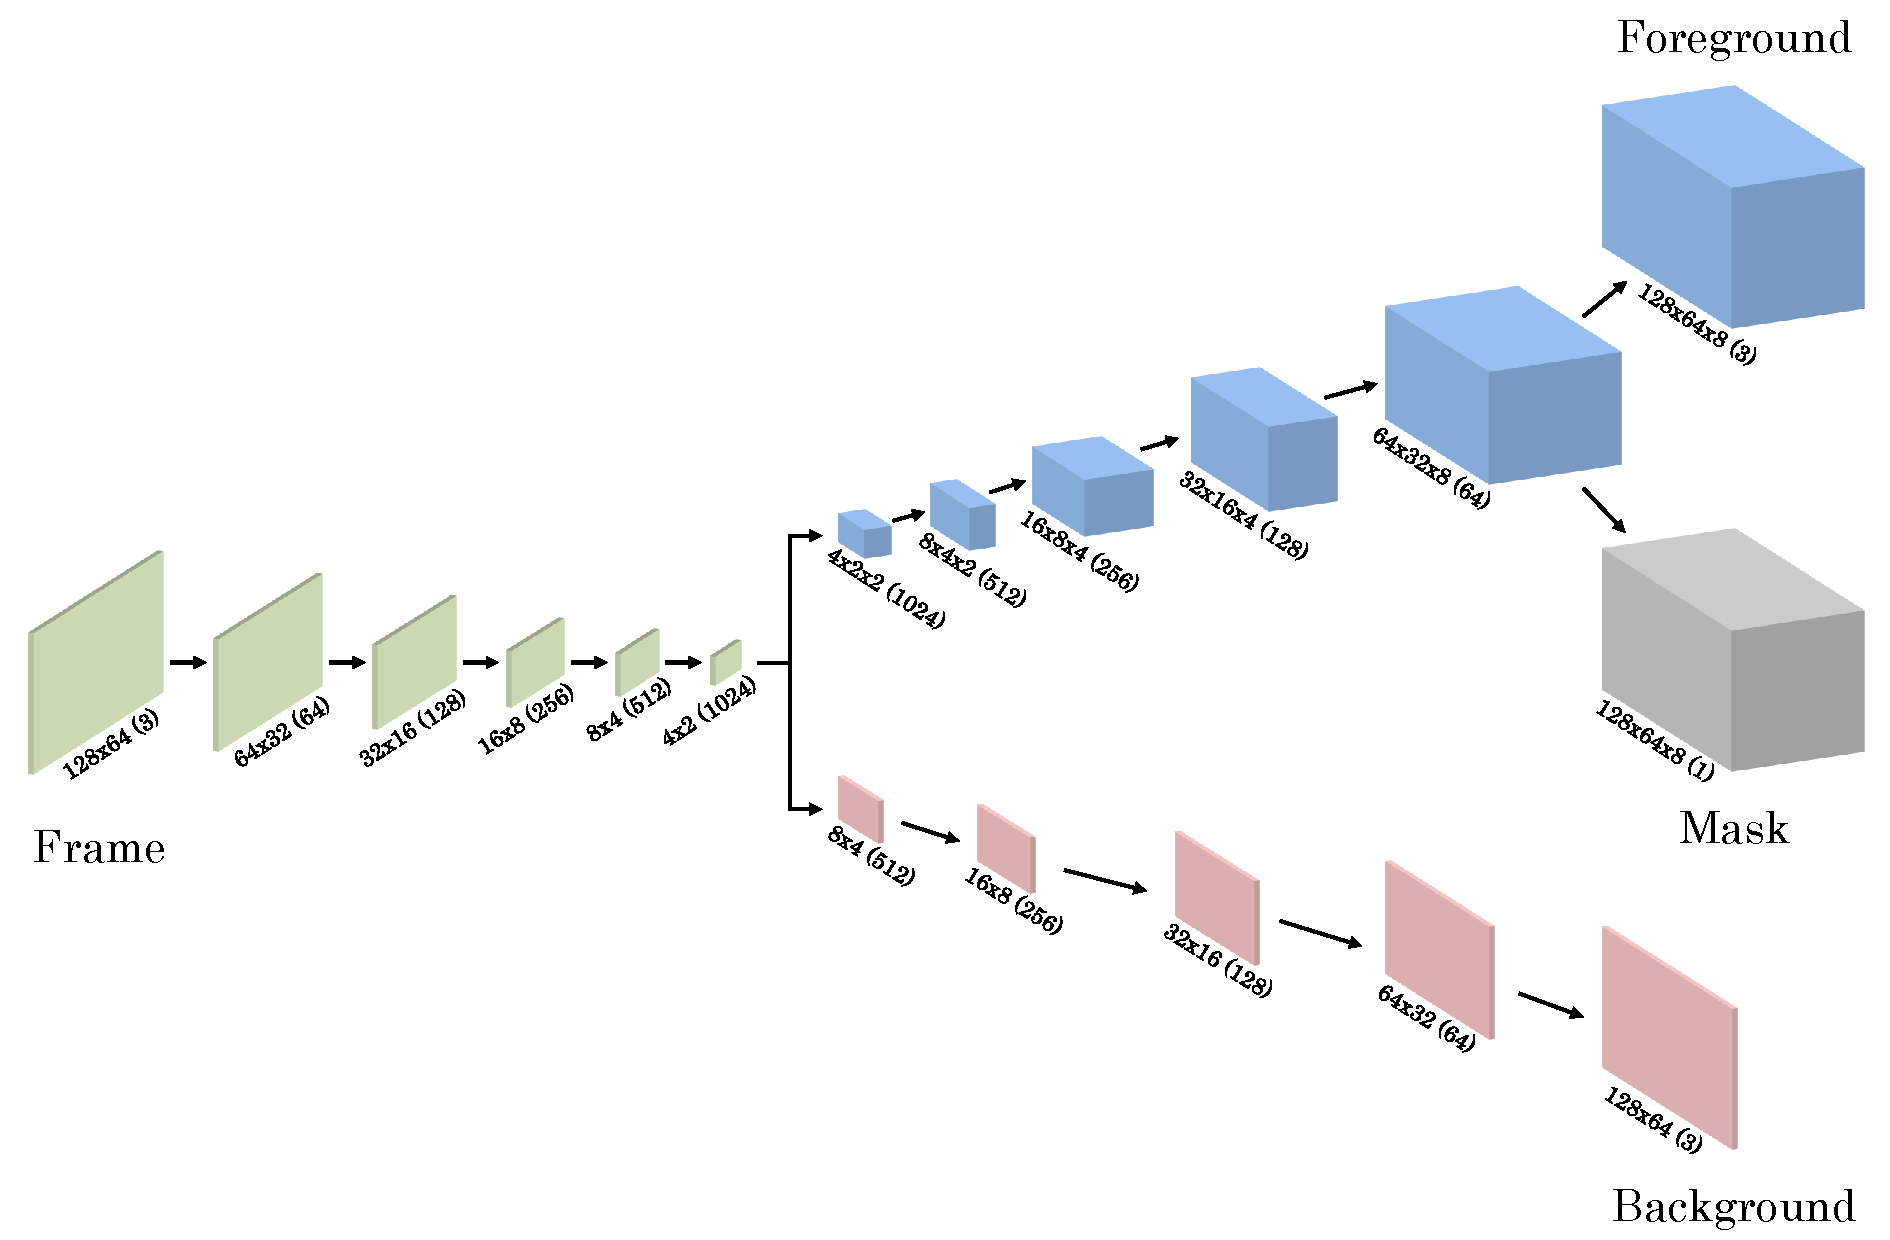
\includegraphics[width=1\textwidth]{graphics/gan/vgan/cvgan_1/cvgan_1.pdf}
  \caption[Adapted video prediction network ($n$ out of $1$ frames).]{Adapted C-VGAN video prediction (generator) network \cite{vondrick2016generating}. Instead of random noise a single frame encoded through strided spatial convolutions to latent space serves as input for the two streams. The rest of the architecture mirrors VGAN, including the combination of foreground, mask, and background to create the generated video output. The number in parentheses is the number of channels.}  
  \label{fig:cvgan_1}
\end{figure}

This minimizes the L1 (Manhattan) distance between the input frame ($x_0$) and the first frame of the respective generated video ($G^0(\cdot)$). $\lambda \in \mathbb{R}$ is a hyperparameter to weight the first frame reconstruction loss with the other two losses. This way, the generator can not simply enter mode collapse, i.e. collapsing different input frames into the same realistic looking output videos. Instead it has to reconstruct the first frame, before learning to generate following frames based on the initial scene. The rest of the generator and discriminator network remain the same.  The resulting model, sometimes called a conditional generative adversarial network for video (C-VGAN) \cite{tulyakov2018mocogan}, was used to extrapolate plausible motions in different scenes. $32$ frames were extrapolated from a single frame beginning that sequence. 

Unfortunately we noticed when inspecting the actual code referenced in the paper by Vondrick et al.\footnote{\url{https://github.com/cvondrick/videogan/blob/master/main_conditional.lua}}, that there were several additional changes done to both the generator and the discriminator without mentioning it anywhere: Not only does the encoder not mirror the background stream --- having only four instead of five convolutional layers, but the number of channels for each convolutional layer was doubled as well. The convolutional filters range from a number of $128$ to $1024$ for the latent space, instead of the expected $64-512$. This also doubled the resulting size of the bottleneck. The rest of the generator was however also altered because of that: Instead of keeping the five layer stack of the two streams, one layer was removed from the background pathway, while the foreground was kept was kept as it was in VGAN. Why these changes were done to the network is not explained anywhere; the version of the code is from the initial commit of that repository. One can assume the widening of the bottleneck and the doubling of the number of filters at every layer were done consciously to avoid the collapse of different inputs to the same generated video. What it does not explain however is the changes for the discriminator. There, the number of convolutional filters was also doubled at every step of the CNN-based classifier. As explained in Section \ref{sec:gans}, this serves to empower the discriminator and prevent the domination of a strengthened generator model. So improving the expressiveness of both models simultaneously is usually the right choice \cite{roth2017stabilizing, zhang2018convergence}.\\

\begin{figure}
	\centering
	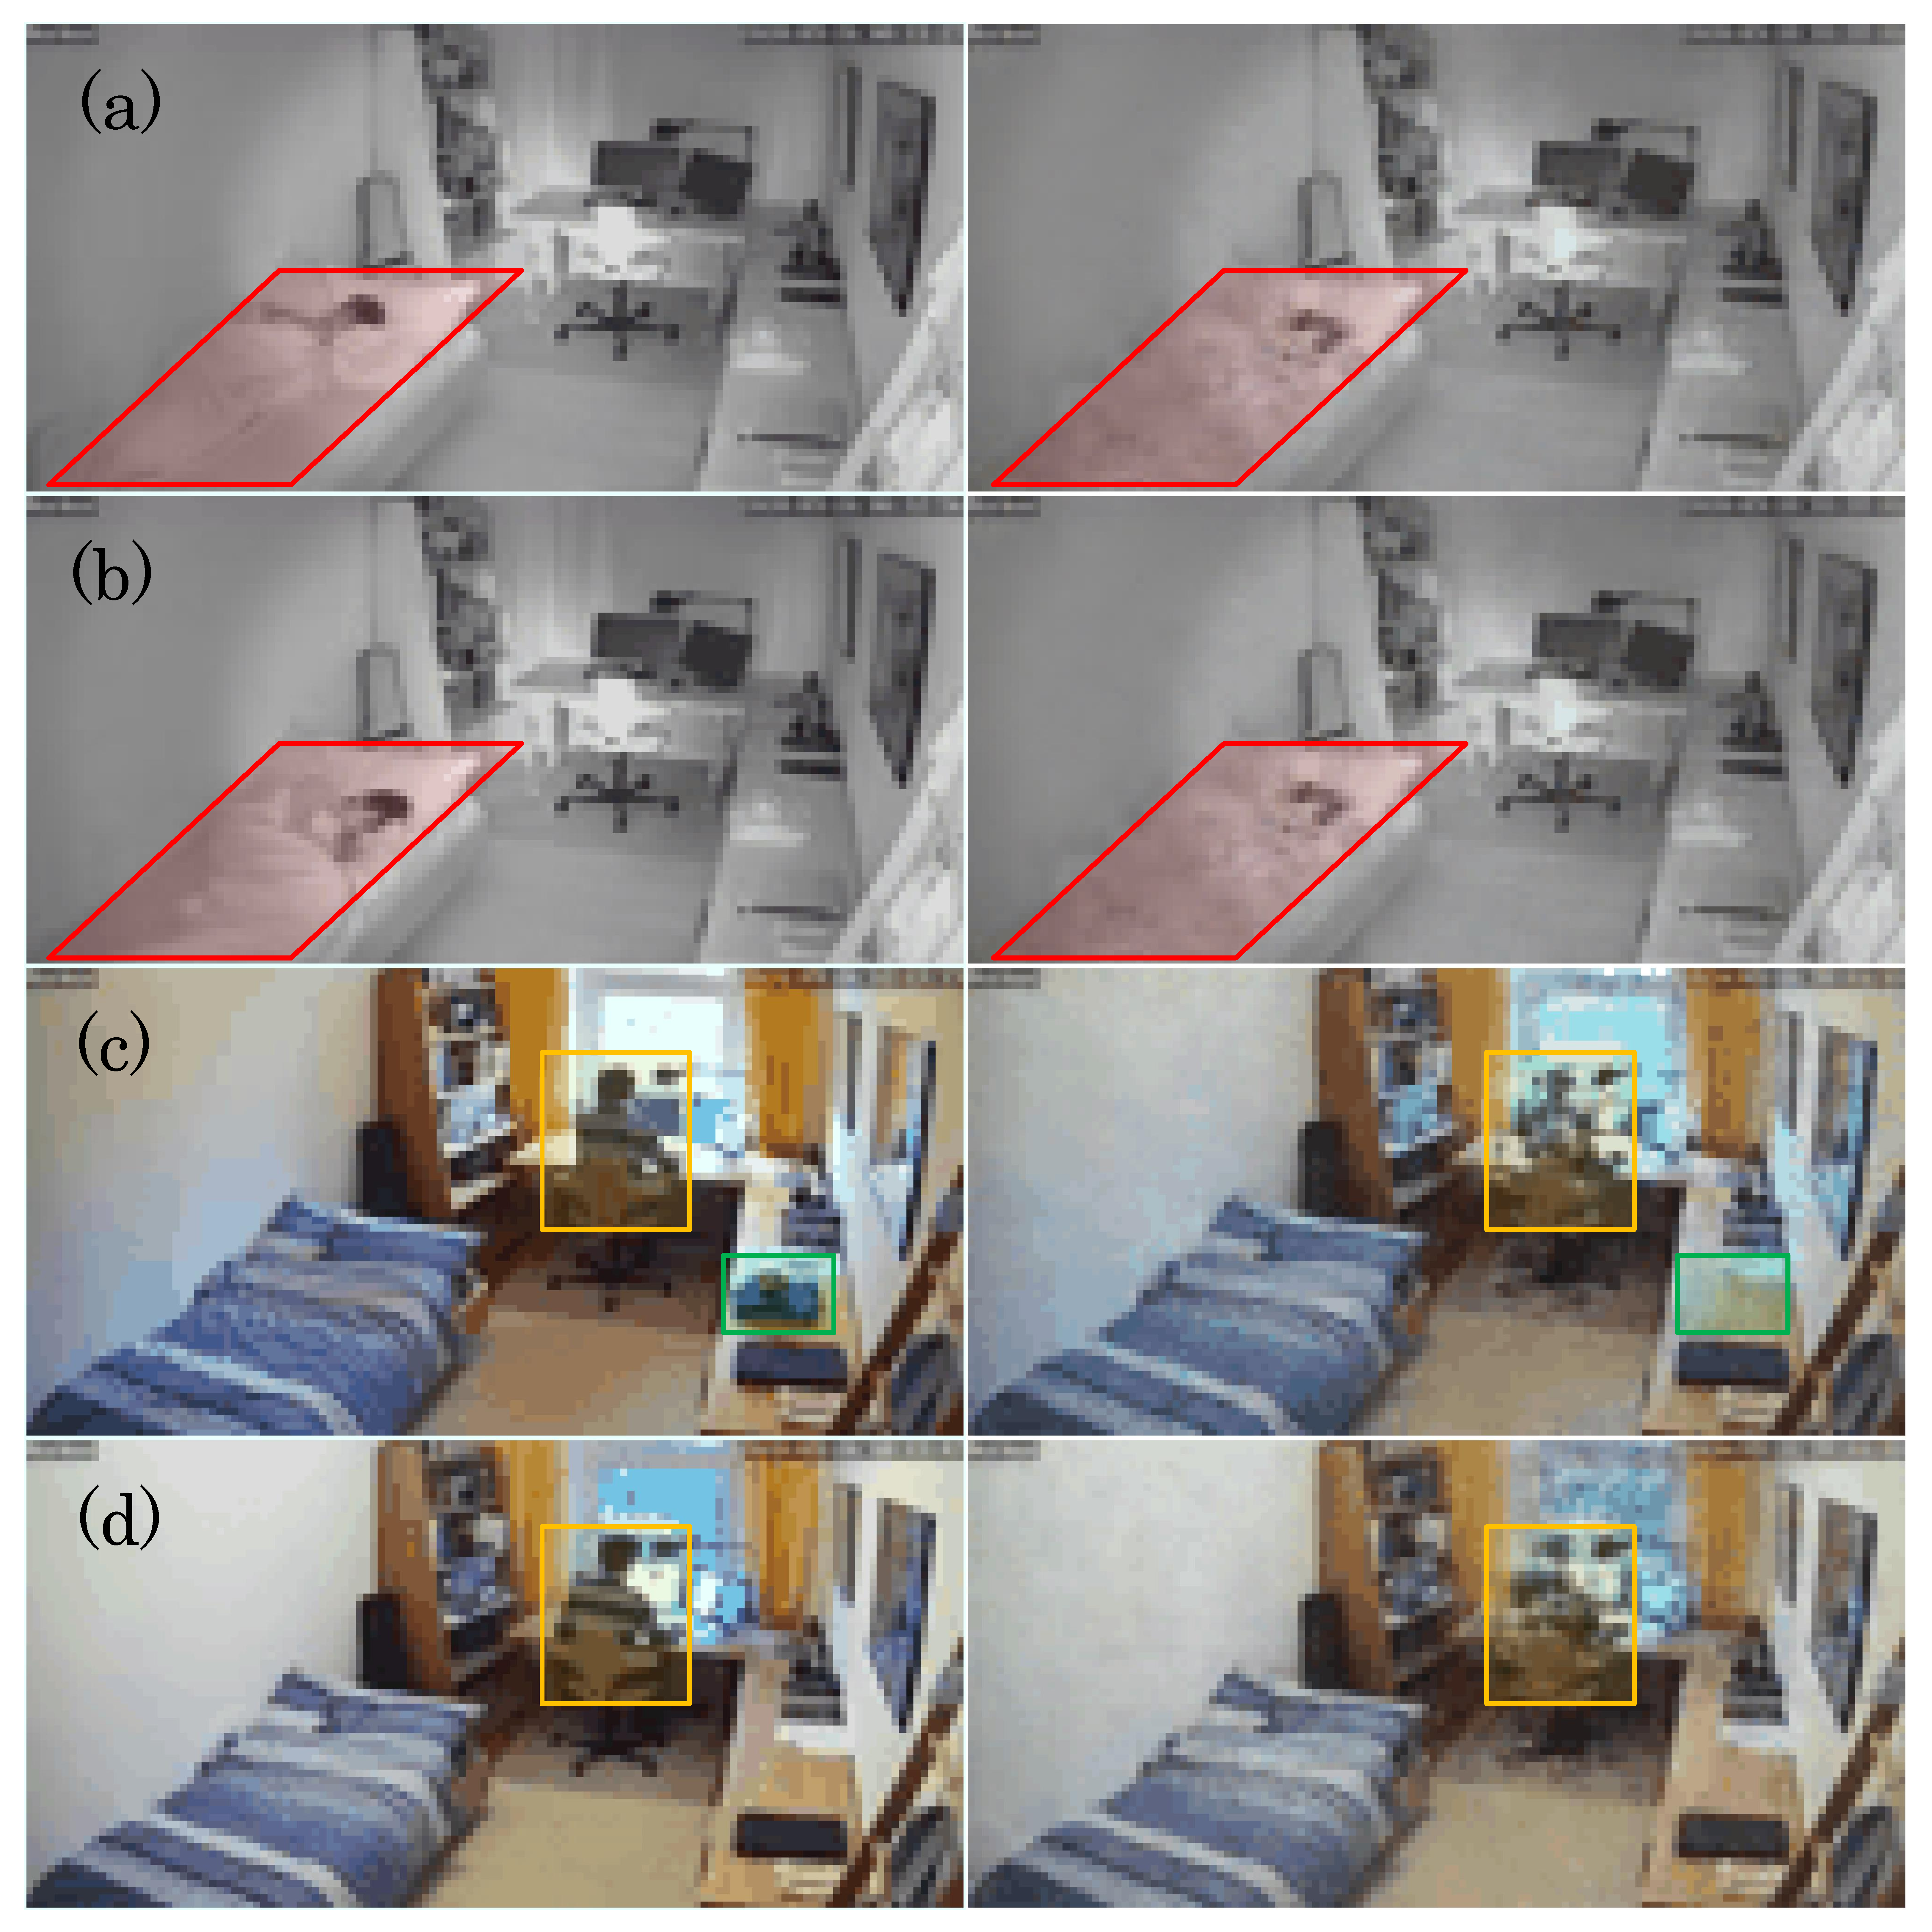
\includegraphics[width=0.6\textwidth]{graphics/eval/cvgan_1/cvgan_1_Collapse.pdf}
  \caption[Comparison between inputs of C-VGAN and their reconstructed outputs.]{First frames that are passed to C-VGAN (left) and the generated first frames (right). Marked in red (a,b) one can see how different object patterns are collapsed into the same pattern during reconstruction. In (c) objects (green) are omitted from the scene entirely. Some object patterns are also not fully reconstructed (yellow), e.g. the person's neck and some of its other features are missing in (d).}
  \label{fig:cvgan_1_out}
\end{figure}

\paragraph{Modifications to C-VGAN}
Due to these ambiguities, when adapting C-VGAN to our data, we first decided to build our interpretation of C-VGAN on our VGAN model described in Section \ref{subsec:vgan_mod} but mix it with the design decisions made in the original C-VGAN code. This results in the generative model depicted in Figure \ref{fig:cvgan_1}: Because our modified models had one additional convolutional layer in each of their streams, the encoder that was attached to our generator has five convolutional layers instead of four. Therefore, the 2D latent space has a size of $4 \times 2$ with $1024$ convolutional filters and both background and foreground upsample from that directly. As the modified VGAN generator, a kernel size of $3$ was used instead of $4$. Because foreground and background stream can directly upsample from the latent space to the next step ($8 \times 4$), doubling the used number of convolutional filters at every step of the stacks, one fractionally-strided convolutional layer was removed from the background. For the foreground stream, the first convolutional layer was instead used to transform the latent code into a 3-dimensional one, using a stride of $2$ along the time axis as in the original C-VGAN. Finally, we kept all of our other modifications to VGAN, such as the weight initialization. The expressiveness of the discriminator was not increased however and it was kept the same.

During our tests with the modified C-VGAN we noticed that even the original discriminator was dominating the modified empowered generator. The empowering of which, by also doubling the number of its convolutional filters as done in the generator, was therefore not necessary. The continued use of the discriminator that was built for VGAN, will be further highlighted in the following section and in Chapter \ref{chap:results}, when we evaluate the different configurations of our final GAN. Other issues we encountered with C-VGAN were similar to the ones Vondrick et al. found. They hint at the bottleneck of the latent space that is still too strong: Forms of mode collapse and the dropping or hallucination (i.e. insertion) of objects were among these. In Figure \ref{fig:cvgan_1_out} one can see the first frames for several different outputs and how the generator model struggles to reconstruct them. Finally, although this model could be integrated into an anomaly detection framework such as IFTM, it is impaired by its very nature: By only using a single frame to predict the future --- not only a single future frame but in our adaptation $7$ frames, the degrees of freedoms for the forecast is too great: While the future may be plausible, it is not likely it will come to pass. In addition, because of our use-case, there is no need to only utilize a single frame as a starting point for forecasting. A continuous stream of video frames is available to the model. Thus in the following section, we adapt C-VGAN to be more constrained during future frame generation.


\subsection{C-VGAN with Spatio-Temporal Input} \label{subsec:vgan_mod_2}

As noted during the modification of C-VGAN and in our use case, the ADS and thus the underlying model as well, have to process frames of the continuous video stream once during the detection phase, one after the other. This is a key difference to the application of VGAN and C-VGAN, that were evaluated using short video clips from Flickr\footnote{\url{www.flickr.com}} \cite{vondrick2016generating}. These clips beside common themes, were usually not directly related to each other, while in our case, the same person appears in many frame windows with similar motion patterns in different contexts. However due to the nature of a single encoder for both generator streams, similar motion and appearance patterns of the same object might be represented differently in the latent space of the generator. This forces the two streams to waste part of their capacity by learning these meaningful features redundantly. This issue was also noticed in later research in video generation \cite{tulyakov2018mocogan, spampinato2018vos, spampinato2019adversarial}, and the solution that was proposed is the further untangling of the two streams in terms of input: Spampinato et al. utilize one traditional latent space for the background stream and a trajectory latent space to ensure spatio-temporal consistence of the foreground \cite{spampinato2019adversarial}, i.e. generating a random latent vector for each of frames that have to be generated (see Section \ref{sec:rel_vgan}). Taking the explicit untangling of the input and transforming VGAN to a next frame prediction model, we propose an extension to C-VGAN to accept spatio-temporal data --- videos, as input. These changes also widen the bottleneck of the generator, which help with the issues that were encountered during the use of C-VGAN.

\begin{figure}
  \centering
  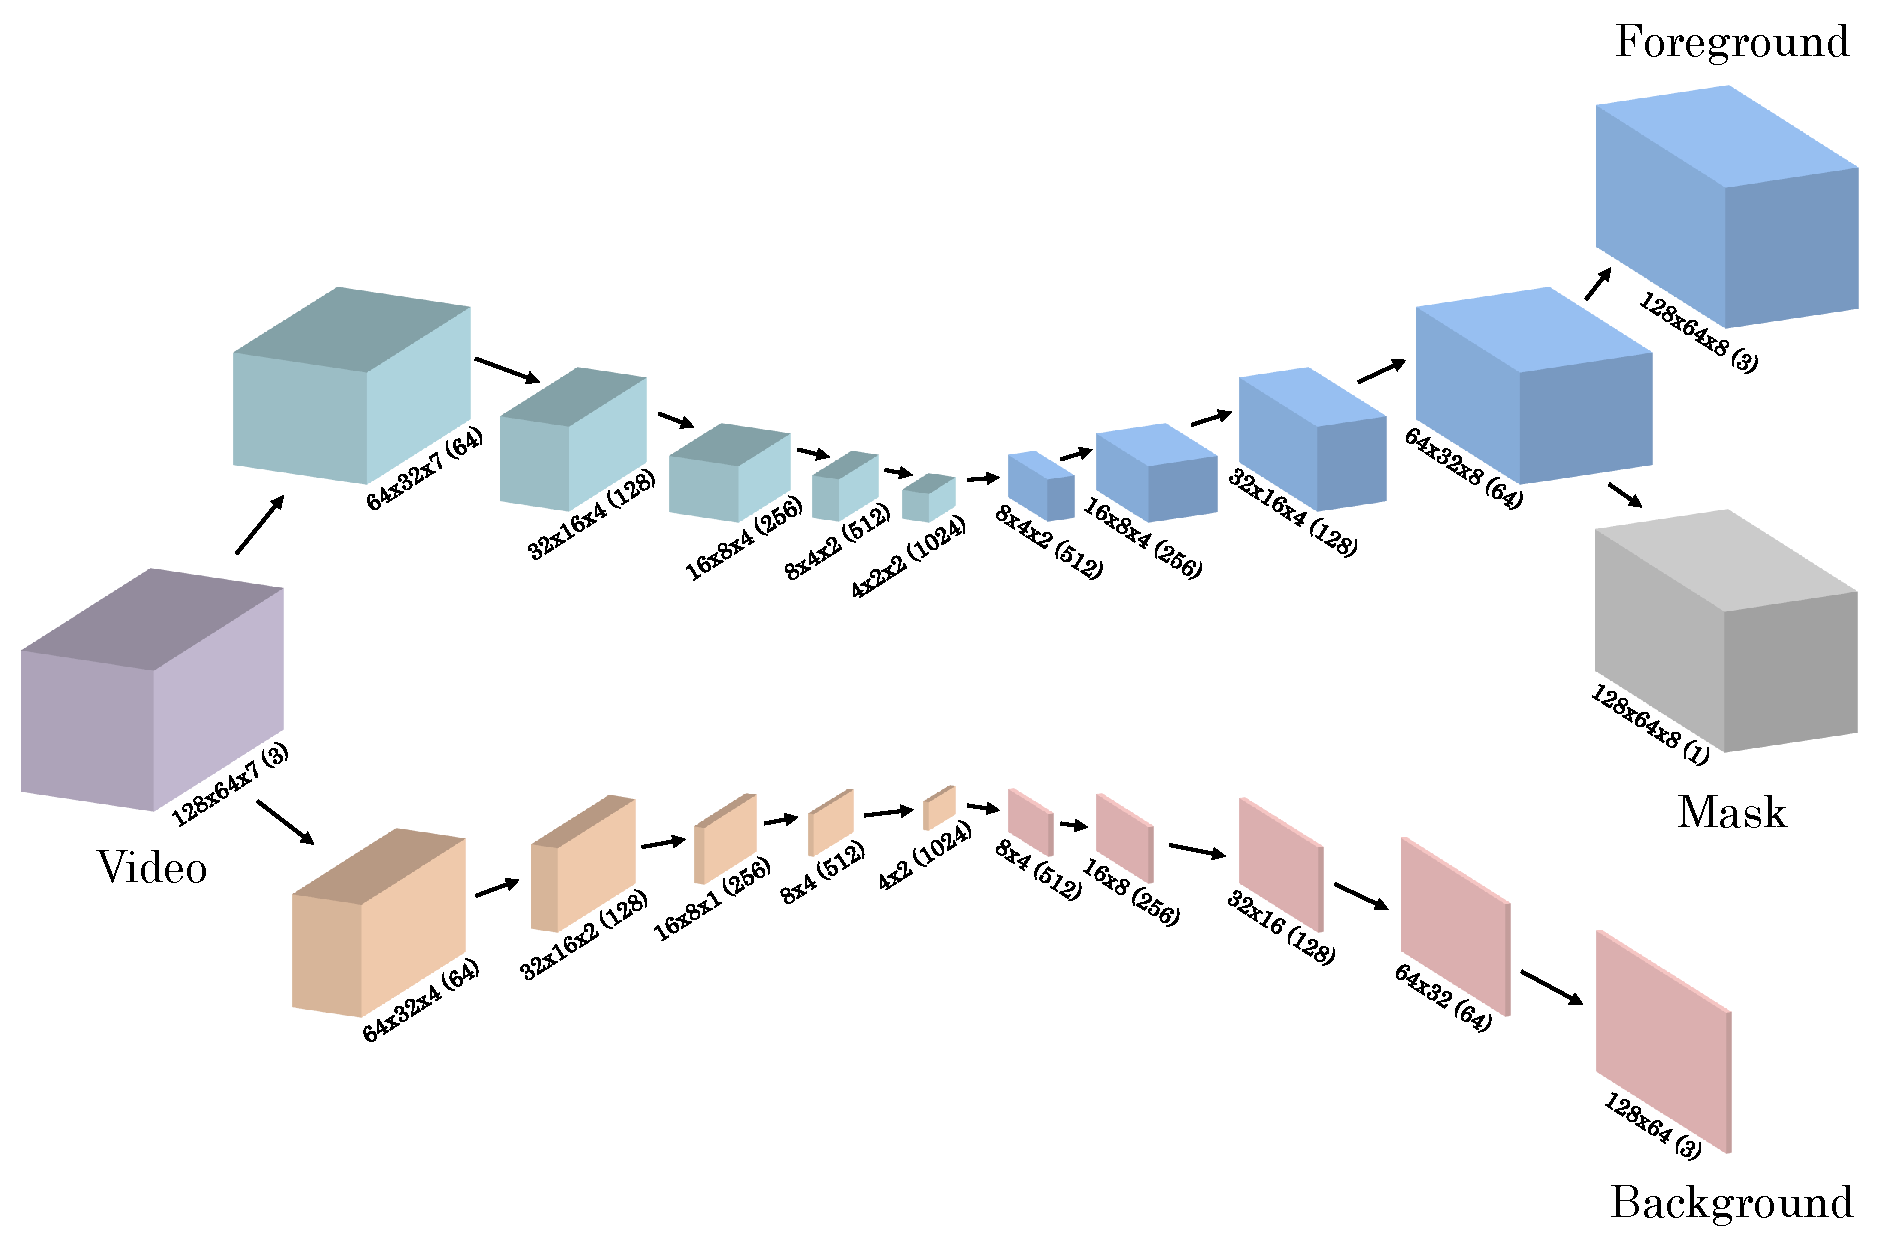
\includegraphics[width=1\textwidth]{graphics/gan/vgan/cvgan_2/cvgan_2.pdf}
  \caption[Next-frame video prediction network.]{Next-frame video prediction (generator) network. Conditional foreground and background stream are further untangled by using different encoders and latent spaces for each of their inputs. Both encoder streams use strided spatio-temporal convolutions, with the background encoder stream falling back to spatial convolutions once the time dimension has been reduced to size 1. The rest of the architecture mirrors VGAN, including the combination of foreground, mask, and background to create the generated video output. The number in parentheses is the number of channels.}
  \label{fig:cvgan_2}
\end{figure}

\begin{table}
	\centering
	\begin{tabular}{ | l | l | l | c | c | c | r !{\makebox[0pt]{$\times$}} r !{\makebox[0pt]{$\times$}} r !{\makebox[0pt]{$\times$}} r |}
	\toprule
	\textbf{\textit{Fg Stream}}			& \textbf{Kernel} 		& \textbf{Stride} 		& \textbf{BN} 	& \textbf{AF} 	& \textbf{Init} & \multicolumn{4}{c |}{\textbf{Output Shape}} \\
	Input 								& $-$  					& $-$  					& $-$  			& $-$  			& $-$ 			& 3 & 128 & 64 & 7		\\
	Conv3D 								& $3 \times 3 \times 3$	& $2 \times 2 \times 1$	& No 			& ReLU 			& He 			& 64 & 64 & 32 & 7		\\
	Conv3D 								& $3 \times 3 \times 3$ & $2 \times 2 \times 2$	& Yes 			& ReLU 			& He 			& 128 & 32 & 16 & 4		\\
	Conv3D 								& $3 \times 3 \times 3$ & $2 \times 2 \times 1$	& Yes 			& ReLU 			& He 			& 256 & 16 & 8 & 4		\\
	Conv3D 								& $3 \times 3 \times 3$ & $2 \times 2 \times 2$	& Yes 			& ReLU 			& He 			& 512 & 8 & 4 & 2		\\
	Conv3D 								& $3 \times 3 \times 3$ & $2 \times 2 \times 1$	& Yes 			& ReLU 			& He 			& 1024 & 4 & 2 & 2		\\
	Conv3DTrans 						& $3 \times 3 \times 3$ & $2 \times 2 \times 1$	& Yes 			& ReLU 			& He 			& 512 & 8 & 4 & 2		\\
	Conv3DTrans 						& $3 \times 3 \times 3$ & $2 \times 2 \times 2$	& Yes 			& ReLU 			& He 			& 256 & 16 & 8 & 4		\\
	Conv3DTrans 						& $3 \times 3 \times 3$ & $2 \times 2 \times 1$	& Yes 			& ReLU 			& He 			& 128 & 32 & 16 & 4		\\
	Conv3DTrans 						& $3 \times 3 \times 3$ & $2 \times 2 \times 2$	& Yes 			& ReLU 			& He 			& 64 & 64 & 32 & 8		\\
	\midrule
	\textbf{\textit{Foreground ($f$)}} 	& \textbf{Kernel} 		& \textbf{Stride} 		& \textbf{BN} 	& \textbf{AF} 	& \textbf{Init} & \multicolumn{4}{c |}{\textbf{Output Shape}} \\
	Conv3DTrans 						& $3 \times 3 \times 3$	& $2 \times 2 \times 1$	& No 			& Tanh 			& Glorot 		& 3 & 128 & 64 & 8 	\\
	\midrule
	\textbf{\textit{Mask ($m$)}} 		& \textbf{Kernel} 		& \textbf{Stride} 		& \textbf{BN} 	& \textbf{AF} 	& \textbf{Init} & \multicolumn{4}{c |}{\textbf{Output Shape}} \\
	Conv3DTrans 						& $3 \times 3 \times 3$	& $2 \times 2 \times 1$ & No 			& Sigmoid 		& Glorot 		& 1 & 128 & 64 & 8 	\\
	TileTensor($3$)						& $-$  					& $-$  					& $-$  			& $-$  			& $-$ 			& 3 & 128 & 64 & 8 	\\
	\midrule
	\textbf{\textit{Bkg Stream ($b$)}} 	& \textbf{Kernel} 		& \textbf{Stride} 		& \textbf{BN} 	& \textbf{AF} 	& \textbf{Init} & \multicolumn{4}{c |}{\textbf{Output Shape}} \\
	Input 								& $-$  					& $-$  					& $-$  			& $-$  			& $-$ 			& 3 & 128 & 64 & 7		\\
	Conv3D 								& $3 \times 3 \times 3$	& $2 \times 2 \times 2$	& No 			& ReLU 			& He 			& 64 & 64 & 32 & 4		\\
	Conv3D 								& $3 \times 3 \times 3$	& $2 \times 2 \times 2$	& Yes 			& ReLU 			& He 			& 128 & 32 & 16 & 2		\\
	Conv3D 								& $3 \times 3 \times 3$	& $2 \times 2 \times 2$	& Yes 			& ReLU 			& He 			& 256 & 16 & 8 & 1		\\
	Conv2D 								& $3 \times 3$			& $2 \times 2$			& Yes 			& ReLU 			& He 			& 512 & 8 & \multicolumn{1}{ r }{4}	&	\\
	Conv2D 								& $3 \times 3$			& $2 \times 2$			& Yes 			& ReLU 			& He 			& 1024 & 4 & \multicolumn{1}{ r }{2} &	\\
	Conv2DTrans 						& $3 \times 3$			& $2 \times 2$			& Yes 			& ReLU 			& He 			& 512 & 8 & \multicolumn{1}{ r }{4} &	\\
	Conv2DTrans 						& $3 \times 3$			& $2 \times 2$			& Yes 			& ReLU 			& He 			& 256 & 16 & \multicolumn{1}{ r }{8} &	\\
	Conv2DTrans 						& $3 \times 3$			& $2 \times 2$			& Yes 			& ReLU 			& He 			& 128 & 32 & \multicolumn{1}{ r }{16} &	\\
	Conv2DTrans 						& $3 \times 3$			& $2 \times 2$			& Yes 			& ReLU 			& He 			& 64 & 64 & \multicolumn{1}{ r }{32} &	\\
	Conv2DTrans 						& $3 \times 3$			& $2 \times 2$			& No 			& Tanh 			& Glorot 		& 3 & 128 & \multicolumn{1}{ r }{64} &	\\
	RepeatTensor($8$) 					& $-$  					& $-$  					& $-$  			& $-$  			& $-$  			& 3 & 128 & 64 & 8 \\
	\bottomrule
	\end{tabular}
	\caption[Architecture of the generator.]{Architecture of the generator: \textit{Fg Stream} lists the layers included in the foreground stream of the model, which is then split into the \textit{Foreground} and its spatio-temporal \textit{Mask}. \textit{Bkg Stream} contains the respective layers of the background stream. The combination of the three tensors is done as described in Equation \ref{eq:vgan}. Note that \textit{Conv3D} stands for strided spatio-temporal convolution, while \textit{Conv3DTrans} stands for its fractionally-strided counterpart. The same is the case for the spatial convolutions used in the background stream. The usage of batch normalization (\textit{BN}), an activation function (\textit{AF}), and the initializer for the kernel weights (\textit{Init}) is also listed per layer.}
	\label{tab:cvgan_arch_g}
\end{table}

\paragraph{Generator}
First for the generator, the single encoder that was attached to the front of the generator in the original C-VGAN is replaced with two separate ones for each stream, which results in the usage of two separate latent spaces. For the encoder that has to create the trajectory latent code to model object patterns for the foreground, a spatio-temporal CNN is attached. Now, instead of a single frame, a sequence of frames are passed to the encoder as input. As with the foreground afterward, convolutional filters range from $64$ to $1024$, using a kernel size of $3$ and a stride of $2$, except for the time axis. The time dimension is again only halved every other step. As shown in Figure \ref{fig:cvgan_2} and described in detail in Table \ref{tab:cvgan_arch_g}, $7$ input frames are passed to the CNN encoder and due to padding during the application of the convolutional filters, the time dimension returns to an even size of $4$ after the second layer. The resulting bottleneck and the trajectory latent space has twice the size of the one in C-VGAN for the foreground alone ($4 \times 2 \times 2$). This is necessary because instead of a preset for a scene for which a video needs to be generated, the information of appearance and motion patterns across multiple frames has to be stored in latent space. Lastly, the first fractionally-strided convolutional layer that was exclusively used in C-VGAN to transform the former spatial latent code into a a spatio-temporal one, is removed.

For the background stream, the encoder is also spatio-temporal at the beginning. Although the background is a static frame that is generated using 2D de-convolutions, the input video --- a space time cuboid, can not be simply flattened or otherwise modified. For example, when using a single frame instead of all $7$ input frames, this results in the loss of information: Static objects in the background might be obscured by dynamic ones. The former objects are thus impossible to be generated by the background stream, because they did not appear in its encoded latent space. These static objects would need to be generated by the foreground instead, that still has the necessary information. But this is not desired. Ideally the background stream is able to generate the entire static part of the scene and the spatio-temporal mask of the foreground stream can show or remove static objects across the frame sequence. Therefore, the first three layers of the background encoder stream are 3D convolutions with a constant stride of $2$ for the convolutional window, so the tensor can be reshaped into a 2-dimensional one (the size of the time dimension is $1$). Afterwards the downsampling to latent code continues using spatial convolutions. This quick reduction of spatio-temporal information in the background encoder stream forces the background to focus on static objects and scenery, while the foreground learns the motion dynamics of non-static objects.

\paragraph{Value Function} \label{par:vgan_mod_2_vfn}
In addition, the loss function during training has to be again extended to account for the reconstruction of all the frames that serve as the input for the generator, as seen in Equation \ref{eq:cvgan_2}. In the case of the displayed generator, $7$ out of $8$ frames ($x_{0;6}$) have to be reconstructed, while the next frame of that sequence has to be extrapolated from them.

\begin{equation} \label{eq:cvgan_2}
\begin{aligned}
\min_G \max_D V(D,G) = & \mathbb{E}_{x \sim p_x(x)}[\log D(x)] + \mathbb{E}_{x_{0;6} \sim p_{x_{0;6}}(x_{0;6})}[\log(1 - D(G(x_{0;6})))] \\
+ & \mathbb{E}_{x_{0;6} \sim p_{x_{0;6}}(x_{0;6})}[\lambda \cdot \|(x_{0;6} - G^{0;6}(x_{0;6}))\|_1]
\end{aligned}
\end{equation}

\begin{table}
	\centering
	\begin{tabular}{ | l | l | l | l | c | c | c | r !{\makebox[0pt]{$\times$}} r !{\makebox[0pt]{$\times$}} r !{\makebox[0pt]{$\times$}} r |}
	\toprule
	\textbf{\textit{Disc.}}	& \textbf{Kernel} 		& \textbf{Stride} 		& \textbf{BN} & \textbf{AF} & \textbf{DO}  	& \textbf{Init} & \multicolumn{4}{c |}{\textbf{Output Shape}} \\
	\midrule
	Input         			& $-$         			& $-$         			& $-$         & $-$ 		& $-$           	& $-$ 			& 3 & 128 & 64 & 8						\\
	Conv3D        			& $3 \times 3 \times 3$ & $2 \times 2 \times 1$ & No          & LReLU		& $dr$	 		& He			& $cf$ & 64 & 32 & 8					\\
	Conv3D        			& $3 \times 3 \times 3$ & $2 \times 2 \times 2$ & Yes         & LReLU		& $dr$	 		& He			& $(2 \cdot cf)$ & 32 & 16 & 4			\\
	Conv3D        			& $3 \times 3 \times 3$ & $2 \times 2 \times 1$ & Yes         & LReLU		& $dr$	 		& He			& $(4 \cdot cf)$ & 16 & 8 & 4			\\
	Conv3D        			& $3 \times 3 \times 3$ & $2 \times 2 \times 2$ & Yes         & LReLU		& $dr$	 		& He			& $(8 \cdot cf)$ & 8 & 4 & 2			\\
	Conv3D        			& $3 \times 3 \times 3$ & $2 \times 2 \times 1$ & Yes         & LReLU		& $dr$	 		& He			& $(16 \cdot cf)$ & 4 & 2 & 2			\\
	Dense         			& $-$         			& $-$         			& $-$         & $-$         & $-$	 		& Glorot 		& \multicolumn{1}{ r }{1} & \multicolumn{1}{ r }{} & \multicolumn{1}{ r }{} &			\\
	\bottomrule
	\end{tabular}
	\caption[Architecture of the discriminator.]{Architecture of the discriminator: As a one-stream CNN, a video is downsampled using strided spatio-temporal convolutions (\textit{Conv3D}) before a single fully connected neuron (\textit{Dense}) gives the binary classification result. The activation function (\textit{AF}) \textit{LReLU} stands for Leaky ReLU and its negative slope coefficient is $\alpha = 0.3$. Batch normalization (\textit{BN}), activation function, and then dropout (\textit{DO}) with a rate of $dr$ is applied to every convolutional layer, in order. The first dimension of each layers output --- the number of channels, i.e. convolutional filters, can be tuned using the $cf$ hyperparameter.}
	\label{tab:cvgan_arch_d}
\end{table}

\paragraph{Discriminator}
Yet this kind of reconstruction loss term comes at a disadvantage: As explained in Section \ref{sec:gans}, the strength of GANs lie in the generator's inability to directly learn from real examples, while the discriminator gives it hints how to fake outputs. This ideally (if there is no mode collapse) allows the generator to generalize well. For example generating similar motion dynamics of objects in video, without ever seeing that kind of motion during training. On the other hand, limiting the degrees of freedom for the generator is necessary due to use video generation for forecasting. This changes the goal of the discriminator in some sense, although the loss term has not been altered explicitly in this manner: $D$ still needs to distinguish real from synthetic videos, but it will quickly learn to ignore the first $7$ out of $8$ synthetic frames for the purpose of discrimination. These frames will appear real because they were reconstructed from real input and the generator learns this through the modified loss term. Now the deciding factor for $D$ is how well the extrapolation from the input frame sequence to the last frame was done. Thus, although the generator has increased in capacity, $D$'s job is actually easier now. This phenomenon is noticed during evaluation in Section \ref{subsec:cvgan_results}, where $D$ overpowers $G$ in a matter of a few epochs. 

Consequently, several options to impair $D$ are introduced: While keeping the overall architecture of the discriminator that was used through the different modification stages, the first impairment parameter is the number of filters for the first convolutional layer and its subsequent layers respectively; following the DCGAN architecture the amount of convolutional filters is doubled with every next convolutional layer. The default value for this hyperparameter ($cf$) is $32$, as that was the configuration that was used during the VGAN and C-VGAN adaptations. Second, regularization layers in the form of dropout layers are added after every layer and its respective activation. The rate of the input units the layers set to $0$ is another set of hyperparameters (default is $dr=0$, no dropout). Further impairment was not required --- the negative slope coefficient ($\alpha=0.3$) of the Leaky ReLU activations used in the discriminator instead of typical ReLU, was also not tuned. An improvement of the generator was also not feasible due to its already high complexity and number of parameters that have to be optimized already. A summary of the model and its parameters can be seen in Table \ref{tab:cvgan_arch_d}.



% Anomaly Detection for Video using IFTM
\section{Anomaly Detection for Video using IFTM} \label{sec:vad}

\begin{figure}
	\centering
	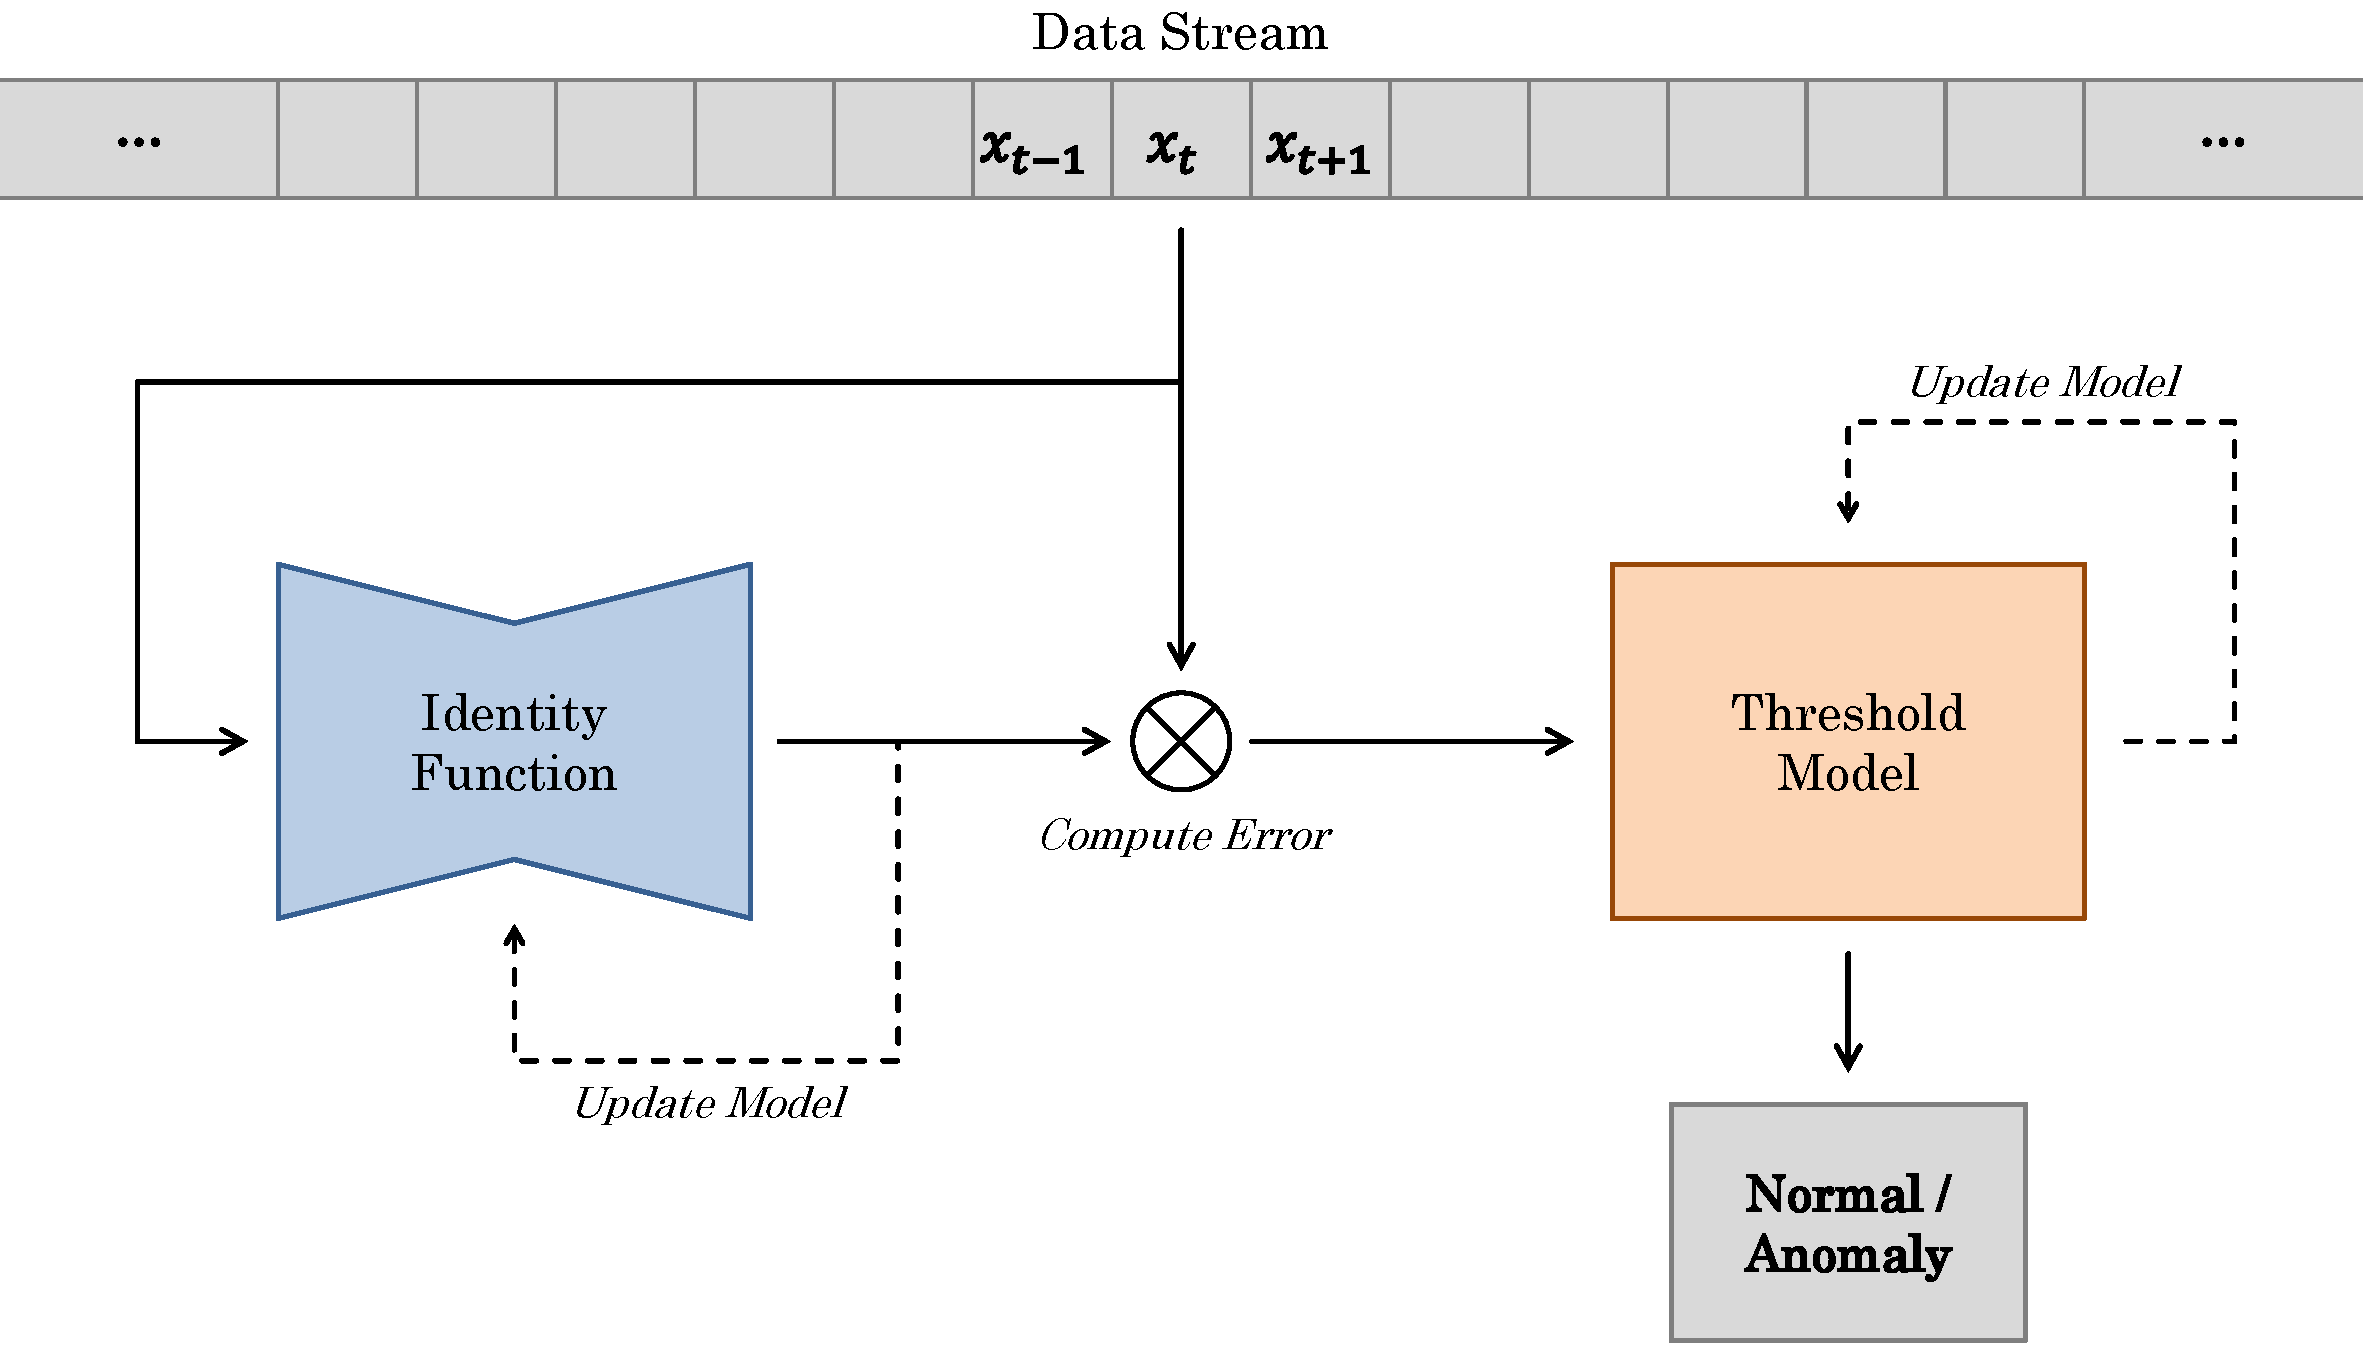
\includegraphics[width=1\textwidth]{graphics/iftm/iftmOriginal/iftmOriginal.pdf}
  \caption[IFTM framework.]{IFTM operating on a data stream. Both identity function and threshold model are trained while making predictions at runtime.}
  \label{fig:iftm}
\end{figure}

As explained in detail in Section \ref{sec:anomaly_detection}, many ADS give the administrator a prediction per event or observation, ranging from $0$ to $1$. This anomaly score describes the model's grade of certainty that a data point is truly an anomaly. Applying a threshold to map this score to a binary result is crucial, but as explained, it is often required that experts set a static threshold for what they consider anomalous. Schmidt et al. solve this challenge through IFTM \cite{schmidt2018iftm}, a framework that combines two components as depicted in Figure \ref{fig:iftm}: The identify function (IF)\nomenclature{IF}{Identity function} serves as the underlying model that computes the anomaly score: Trained in unsupervised manner, the IF is supposed to model the properties of the normality of the data stream, while being unable to model anomalous observations. As the name suggests, Schmidt et al. use the identity function $s: X \rightarrow X$ with $x \in X$ being a single observation in the stream. $s$ is approximated by using the observations witnessed in the past in online fashion. And because it is assumed that the stream is mostly normal in nature, $s$ is able to reconstruct normal observations more easily. The reconstruction of $s(x)=x^{\prime}$ when $x$ is anomalous however should have a higher reconstruction error $\Delta$, because the model is unable to model its properties:

\begin{equation} \label{eq:recon}
\Delta(x) = ||x-s(x)||_2
\end{equation}

For the IF, any kind of model that supports reconstruction can be used, including models from the field of deeplearning. Reconstruction can also be replaced by a forecasting model, as Schmidt et al. suggest. Instead of computing the reconstruction shown in Equation \ref{eq:recon} and minimizing it during training, the model instead has to learn to predict the next observation of the stream, $x_t$. As shown in Equation \ref{eq:forc}, the prediction and therefore the prediction error this time is done on a number of past observations. Because IFTM is abstract by design, the underlying forecasting model could be anything and therefore could use the past in different ways. For example, one could use a type of recurrent neural network (RNN)\nomenclature{RNN}{Recurrent neural network}, such as long short-term memory (LSTM)\nomenclature{LSTM}{Long short-term memory} units, that dynamically learns to ignore certain inputs or forget past ones \cite{hochreiter1997long}.

\begin{equation} \label{eq:forc}
\Delta(x_{t}) = ||x_{t}-s(x_{0;t-1})||_2
\end{equation}

Due to the IF being ideally trained in online manner --- it should be able to adapt to new contexts and normal properties of the data stream, the meaning of a specific anomaly score can also change over time. But one still has make the binary discrimination at the moment the observation occurs. Therefore, Schmidt et al. propose a second model that represents the threshold $T$, that is applied to $\Delta(x)$, the threshold model (TM)\nomenclature{TM}{Threshold model}. If the reconstruction or forecasting error is greater than $T$, it is considered an anomaly. As $s$ adapts to the data stream, $T$ has to adapt with it and is therefore also trained in an unsupervised online manner. Assuming $\Delta$ is normally distributed, $T$ for a given data stream can be defined with the following:

\begin{equation} \label{eq:tm}
T = \mu(\Delta) + \sigma(\Delta)
\end{equation}

\begin{figure}
	\centering
	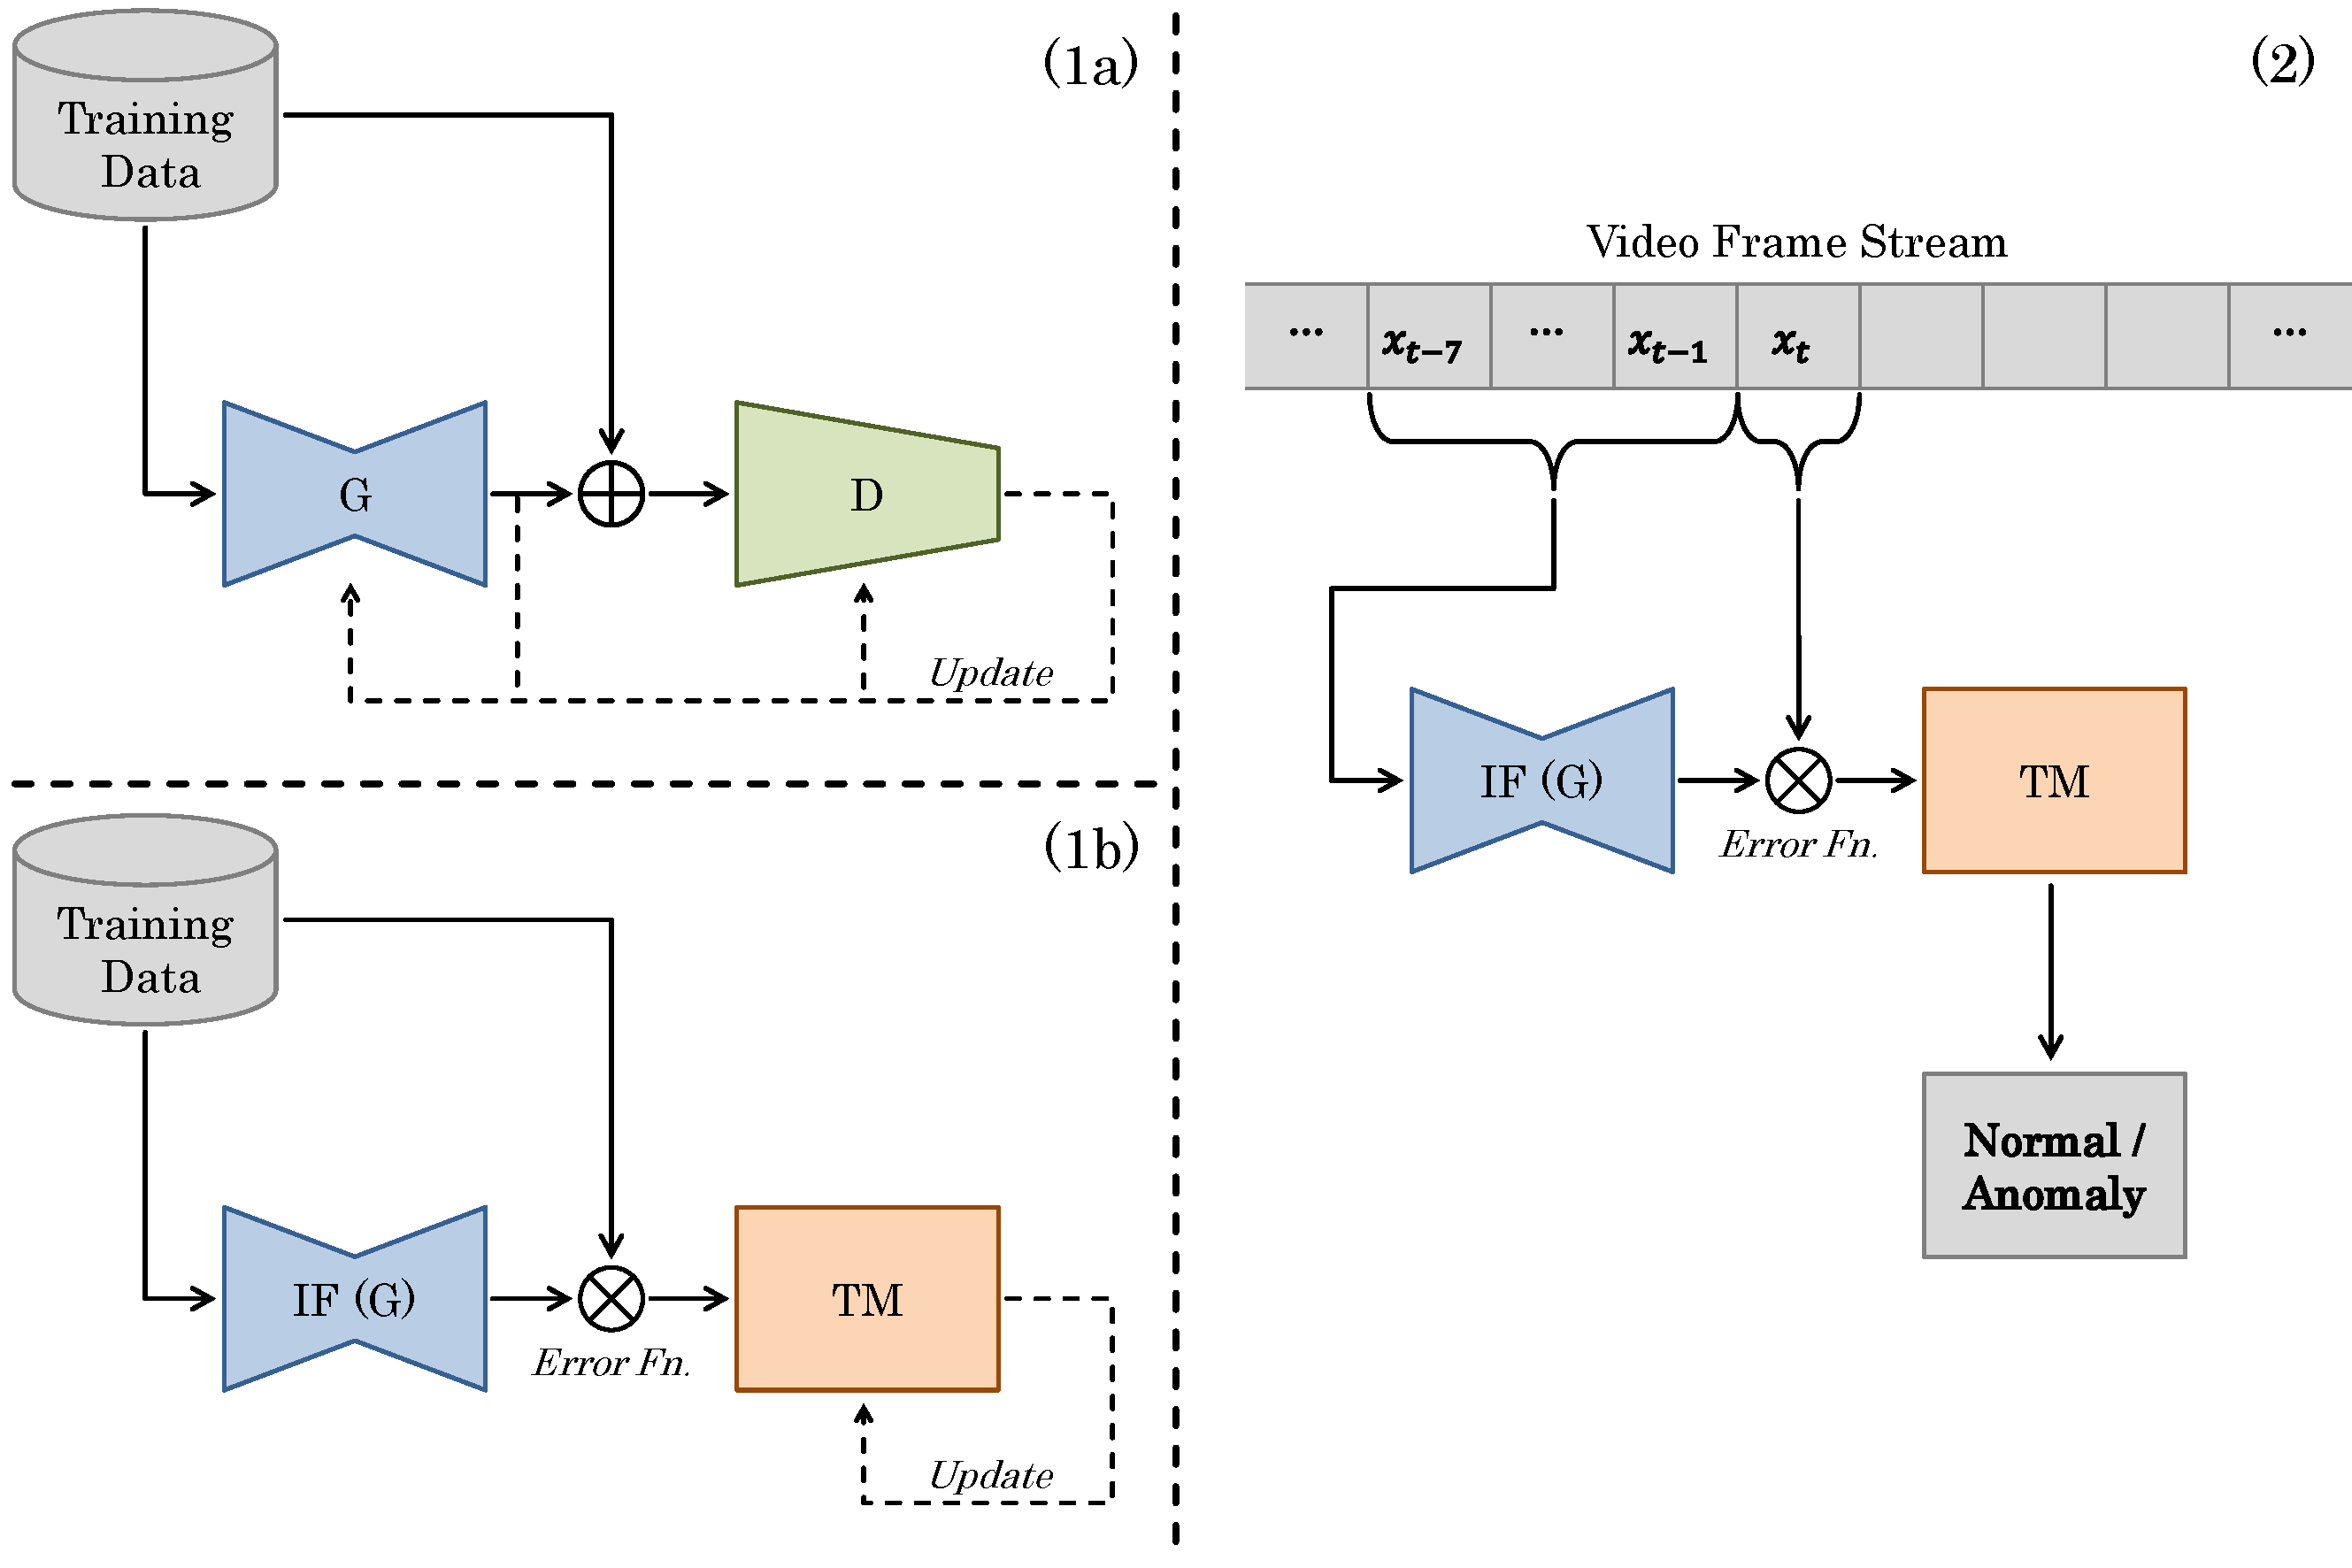
\includegraphics[width=1\textwidth]{graphics/iftm/iftmModified/iftmModified.pdf}
  \caption[IFTM framework adapted for video generation forecasting.]{IFTM framework adapted for video generation forecasting, by splitting training and prediction into separate phases: (1a) features the training of the C-VGAN next-frame video prediction generator network (\textit{G}) and its discriminator (\textit{D}), following the GAN training loop. In (1b) the threshold model (\textit{TM}) is trained using the training data and the trained generator model as identity function (\textit{IF}). In the second phase (2), IFTM makes next-frame video prediction on the stream, labeling frames as either normal or anomalous.}
  \label{fig:iftm_video}
\end{figure}

How the mean ($\mu$) and the standard deviation ($\sigma$) is computed depends on the use case. First, one can compute these two iteratively over the entire data stream online. This kind of cumulative aggregation of two values is not stable however with longer periods of time because the past will dominate $T$ as newer values have less weight assuming an infinite stream. Alternatives present themselves in the form of sliding window aggregations and moving averages in which older data points of the stream are discarded from the distribution. One can also compute $T$ using other techniques but for the sake of our approach, it is assumed that the reconstruction error follows a normal distribution and $T$ can be defined using the equation above.

\paragraph{IFTM with Video Generation Forecasting}
Assuming that a video generation model trained on mostly normal data will model the normal properties of video while being unable to find a representation for anomalous video frames, we propose an integration of our adapted C-VGAN for next-frame video forecasting into IFTM to perform VAD. This requires some modifications to IFTM: First for C-VGAN the reconstruction of past frames is done using the Manhattan (L1) distance and not the Euclidean (L2) distance, as described in the previous section. This also indirectly defines the properties of the forecast frame. So when computing the prediction error for a forecast video frame the L1 metric is utilized. Also, our adapted C-VGAN next-frame prediction network in the configuration presented uses a fixed number of past frames ($7$) to predict the next one. This results in the following adjusted prediction error function:

\begin{equation} \label{eq:forc_2}
\Delta(x_{t}) = ||x_{t}-s(x_{t-7;t-1})||_1
\end{equation}

Second, as explained in Section \ref{sec:gans}, training of any GAN is never done online but done on the entire training data set available. Splitting the data into smaller equal-sized mini-batches, the two models are optimized in min-max fashion until a somewhat stable convergence of their losses is achieved and satisfactory synthetic values are generated. This can require dozens if not hundreds of iterations --- also called epochs, over the entire data set. Because it is not feasible to do the training of the GAN online, neither the TM is trained online. Thus, both forecasting model and TM operate as displayed in Figure \ref{fig:iftm_video}: During the (offline) training phase, the GAN is first trained in usual manner until convergence is achieved. Then, the entire training set is re-run on the generator model to compute the prediction errors and the resulting mean and standard deviation of the errors over the training set. Then in the detection phase, when running on the unknown data stream, forecasting, computation of the error, and the application of $T$ is done online. Note that when training IFTM this way, the framework will no longer have the ability to react to context shifts over time. The underlying prediction model has to learn all properties that normal data can have during the offline training phase, taken it has enough capacity to learn all these features. This does not matter for our our evaluation of IFTM for video though, because the data comes from a single camera source over a variety of days and the labeled evaluation data is from the same time frame. There is no noticeable context shift over that time span. How the data sets were created, labeled, and how they are structured will be explained in the following section.



% Dataset
\section{Data Set} \label{sec:dataset}

In this section, the large-scale data set for VAD evaluation, that was already touched upon in the use case in Section \ref{sec:use_case}, is presented. We provide insight into how the data set is structured and what properties it has. For the labeled video data, an analysis based on the kind of normal and anomalous frames in it is done. This includes statistics regarding the balance of the two classes. Lastly, the different steps that were taking during preprocessing of the video files are mentioned and the reason why they were taken are explained.


% Creation of Dataset, Underlying Structure
\subsection{Properties} \label{subsec:dataset_properties}

To create a large quantity of video data for anomaly detection using video generation, a camera was positioned in a home office room to monitor it over several days. Capturing the video with a resolution of $640 \times 352$ and varying frame rate of $2.5$ to $5$, the view is static; in position, viewing angle, direction, and field of view. During the night, the fps is reduced by the camera automatically due to switching to a grayscale night vision mode. In addition, a timestamp containing the date and the time is in the top right corner of every video frame.

\begin{figure}
	\centering
	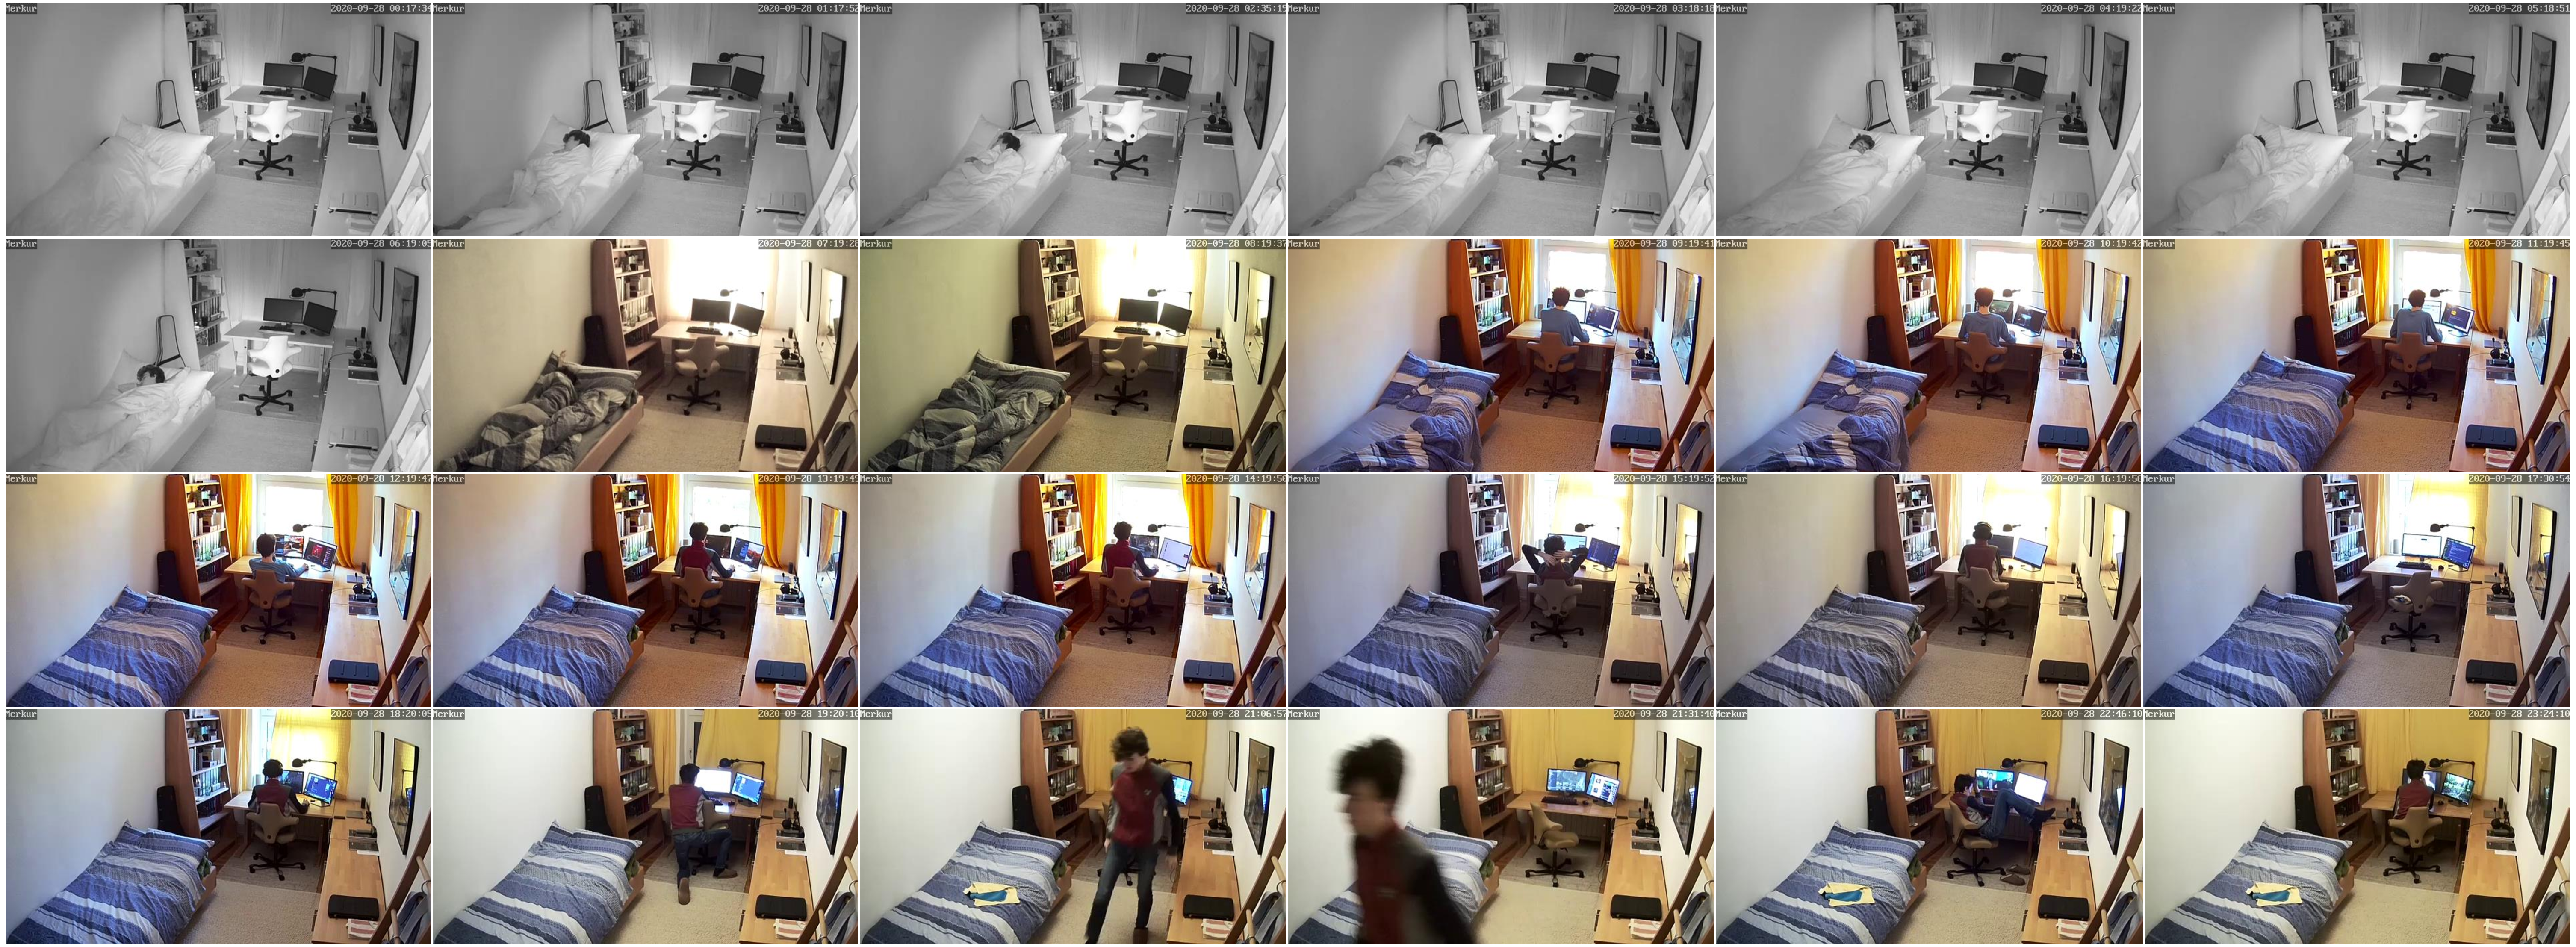
\includegraphics[width=1\textwidth]{graphics/cctv/oneDay/oneDay.pdf}
  \caption[Monitored room during different hours of the day]{Monitored room during the different hours of one of the captured days.}
  \label{fig:room_frames}
\end{figure}

\paragraph{Training Data}
For collecting the unlabeled but assuming mostly normal video data set, monitoring was done atleast for a day to create one part of the data set, generating 24 one hour long videos (MP4 format). Furthermore, capturing was done in bulk, five days each during September and November of 2020, respectively. In Figure \ref{fig:room_frames} frames of each of the 24 hours of one of the monitored days are shown. As one can see, the scenery does not change much overall --- the person usually works at the desk and sleeps in the bed behind them during the night when the light is turned off. Although the person moves around, enters and leaves the room from time to time, the video is often static. This offers any VAD an additional challenge, because the video is unfiltered: Depending how the data set is used during training, a model has to refrain from collapsing into a naive motion detector that considers any kind of movement and abrupt change as anomalous behavior. It has to learn to identify ``idle`` intervals in the video, in which for example the person is sleeping or the room is empty for several hours in a row, and quickly understand the normal contents of such, while also being able to recognize normal motion patterns of objects as for what they are. Differentiating these from anomalous ones is the challenge. Furthermore, the clothing of the person in the room does usually only change twice for a single day. When getting out of bed the clothing changes to day clothes until night, where they switch back to pajamas. Both sets of clothing are not constant across different days however --- the person is not wearing the same kind of clothes every day, so any model should learn to ignore these features and not directly learn them. Else frames in which the person wears unknown clothing will be more likely to be considered anomalous. 

Motion dynamics alone are not the only events of interest to a VAD for our data set: The scenery changes dynamically over the day, as shown in the figure, and this adds lots of contextual information to the scene: For example, during the day, the curtains are open and the person either walks around the room or sits at their desk. As the lighting in the morning increase, at one point the grayscale image switches to the colored view due to the camera adjusting to day-mode. In the evening, the curtains are closed when it gets darker outside, but as long as the light is on, the person still is active in the room. This changes when the light is turned off, as the monitored person goes to bed. This part of the information that has to be extracted is periodic in nature due to the 24-hour cycle and a VAD should be able to model this periodic rhythm. 

The motion patterns of objects are also determined on the context: Lying still in bed is considered normal during the night, but an unusual behavior during the day. Lying on the floor or on the cupboard is also very anomalous no matter the circumstances. But, the line between the two classes become blurry, when there are rare but normal motion patterns that do not appear often during the day. Sitting on the bed for some minutes or standing around in the room, should be considered normal behavior. But due to their rarity, a VAD that has to forget anomalous observations encountered during training to ensure it only contains the normal features of the video, might forget these rare events as well, if it is unable to model similar motion dynamics in the right contexts appropriately.

\paragraph{Evaluation Data}
When building the labeled evaluation set, monitoring was fixed to a single hour. To inject a variety of anomalies into that hour, events were created in quick succession. An event in this case describes a subset of the stream of frames that are somehow related to each other. An event can either be considered normal or anomalous. For example, when standing up and walking through the room, in the video there is a number of frames that contain this event and these frames would each be labeled as normal ones. The events generated range from a second to several minutes, thus being 5 frames to a few thousand frames long. As this set is one hour long, it contains $\sim 18,000$ frames when using a stabilized frame rate (see the next section regarding preprocessing). 

\begin{table}
	\centering
	\begin{tabular}{ | l | c | c | p{9.5cm} |}
	\toprule
	\textbf{Frames} & \textbf{MD} & \textbf{Lights} & \textbf{Normal Event Description} \\
	\midrule
	$00001 - 01557$ & Yes & On & Working at desk, before standing up, leaving room. \\
	$01558 - 01876$ & No  & On & Room left empty. Computer display turned on. \\
	$01877 - 02389$ & Yes & On & Entering the room, walking around. \\
	$02743 - 02831$ & Yes & On & Working at the desk without sitting down. \\
	$03270 - 03666$ & Yes & On & Turning off displays, leaving/entering room. \\
	$03667 - 03672$ & Yes & On & Sitting down at desk. \\
	$04170 - 05420$ & Yes & On & Person turning on displays, then working. \\
	$06861 - 07337$ & Yes & On & Walking around, miscellaneous interactions with room, and leaving/entering room multiple times. \\
	$07338 - 08109$ & Yes & On & Person sitting down at desk, before getting up again, and then leaving room. \\
	$09720 - 09775$ & No  & Off  & Room empty. \\
	$09776 - 10249$ & Yes & Off  & Person entering room, going to bed, and then sleeping. \\
	$10371 - 10509$ & No  & Off  & Room empty. \\
	$10537 - 10608$ & Yes & On 	 & Person walking around, interacting with objects. \\
	$10729 - 11305$ & No  & Off  & Sleeping person in bed. \\
	$11460 - 11924$ & Yes & Off  & Person returning to bed, sleeping. \\
	$11925 - 11970$ & Yes & On   & Person getting up from bed, leaving room. \\
	$12019 - 13959$ & Yes & On   & Working at desk, sometimes getting up, walking around. \\
	$14139 - 14269$ & Yes & On   & Person walking around room before leaving room. \\
	$14270 - 15641$ & No  & On   & Room empty. \\
	$15642 - 16890$ & Yes & On   & Person entering room with different clothing, working, and walking around. \\
	$16893 - 16896$ & No  & On & Room empty. \\
	$17165 - 17168$ & Yes & On & Person leaving room. \\
	$17429 - 18066$ & Yes & Off  & Person returning to bed, sleeping. \\
	\bottomrule
	\end{tabular}
	\caption[Normal events in the evaluation data set.]{Normal events in the evaluation data set sorted by the \textit{Frames} in which they occur. Some events take place while the room is lit (\textit{Lights}) others while the lights are turned off. Not every event has to contain motion dynamics (\textit{MD}); sometimes the room is empty or the person is not moving at all.}
	\label{tab:dataset_normal}
\end{table}

First, for the $5,517$ normal frames, displayed in Table \ref{tab:dataset_normal}, it is to note that that the evaluation data set was created during the evening while it was dark outside. This was done due to the need of artificial light and the closed curtains, which allows us to create many different events. During a normal evening in the home office, the monitored person usually works at the desk, sometimes paces through and out of the room, until eventually going to bed when the lights are turned off. The created normal events mirror that, but with variations to the training data set, e.g. the clothing the person is wearing is different and switches during the evaluation video. In addition, the density of events containing motion dynamics is also higher, to cover the different object patterns that occur over the entire training data set during the evenings and to challenge any VAD model that collapses into a motion detector, labeling every motion pattern as anomalous. This results in some events that usually only appear once during the evening to appear multiple times, while some of them are cut short or left out entirely. For example, it is impossible to have an entire sleep cycle in a labeled data set due to the length of that event that also has little motion dynamics in it, which would also imbalance and skew with the results.

\begin{table}
	\centering
	\begin{tabular}{ | l | c | p{11cm} |}
	\toprule
	\textbf{Frames} & \textbf{Lights} & \textbf{Non-Contextually Anomalous Event Description} \\
	\midrule
	$03136 - 03269$ & On & Person sitting on the edge of the bed, without getting up. \\
	$03673 - 04169$ & On & Person pretending to work at desk, without turning displays on. \\
	$05421 - 05810$ & On & Person moving with chair to middle of room. \\
	$05811 - 05917$ & On & Standing up, leaving chair in middle of room. \\
	$05918 - 06352$ & On & Person kneeling down at desk, chair not at desk. \\
	$06353 - 06440$ & On & Person pacing through room, chair not returned to desk.  \\
	$06441 - 06468$ & On & Pushing chair out of the frame. \\
	$06469 - 06776$ & On & Climbing from chair onto low-board, jumping down from it. \\
	$06777 - 06828$ & On & Person running around room erratically. \\
	$06829 - 06860$ & On & Person moving chair back to desk. \\
	$08110 - 08115$ & $-$ & Turning off lights. \\
	$10510 - 10536$ & $-$ & Turning on lights. \\
	$10696 - 10722$ & $-$ & Turning off lights. \\
	$11971 - 12000$ & $-$ & Turning on lights. \\
	$12001 - 12018$ & On & Pretending to work at desk, without turning displays on. \\
	$17096 - 17164$ & On & Person standing up, moving around erratically. \\
	$17169 - 17218$ & $-$ & Turning off lights. \\
	\bottomrule
	\end{tabular}
	\caption[Non-contextual anomalies in the evaluation data set.]{Non-contextual anomalies in the evaluation data set aggregated by event and their \textit{Frames} in which they occur. All of these either occur when the \textit{Lights} are turned on, or when the lighting of the room changes.}
	\label{tab:dataset_nc_anomaly}
\end{table}

On the other hand for the anomalous events that range a total of $12,549$ frames, a different approach to generate the events was attempted. As explained in Section \ref{subsec:anomaly_types}, in which the three types of anomalies was reiterated upon, we first divided our events that are to be generated into two classes: First, non-contextual anomalies cover motion patterns that should be detected by their patterns alone and without any contextual information that would need to be extracted. See Table \ref{tab:dataset_nc_anomaly} for these kind of events in the evaluation set. Because anomalous motion dynamics of interest do not occur during the night when the lights are turned off --- these could be detected using the contextual features, these anomalies are collective in nature, with a few exceptions. For one, switching on and off the lights forces the camera to quickly adjust its lighting settings which creates lots of noise and thus frames that on their own would be considered point anomalies. Others, such as the monitored person sitting on the edge of the bed can occur in normal events, however the person does not sit there for long under normal circumstance, but they should get up quickly. Other events contain motion dynamics that would be considered normal, if they were to occur in certain regions of the frame or with another motion dynamic preceding them. Sitting at the desk and turning displays on would be normal, while sitting down and keeping the displays turned off would be not. The speed of a object motion pattern also matters. If the person moves through the room too quickly or if they move their arms in erratic fashion, it becomes an anomalous event.

\begin{table}
	\centering
	\begin{tabular}{ | l | c | c | p{9.5cm} |}
	\toprule
	\textbf{Frames} & \textbf{MD} & \textbf{Lights} & \textbf{Contextually Anomalous Event Description} \\
	\midrule
	$02390 - 02742$ & Yes & On  & Person lying on bed, before getting up again. \\
	$02832 - 03135$ & Yes & On  & Person lying on bed, before getting up again. \\
	$08116 - 08913$ & Yes & Off & Person pacing through room, before returning to desk. \\
	$08914 - 09065$ & Yes & Off & Person pacing through room. \\
	$09066 - 09135$ & Yes & Off & Person is climbing from chair onto low-board, jumping down from it. \\
	$09136 - 09161$ & Yes & Off & Person working at the desk without sitting down, afterwards pacing through room. \\
	$09162 - 09589$ & Yes & Off & Person sitting on the edge of the bed, then lying down. \\
	$09590 - 09695$ & Yes & Off & Standing up, walking to desk, turning off displays. \\
	$09696 - 09719$ & Yes & Off & Person leaving room. \\
	$10250 - 10370$ & Yes & On  & Getting up, then making bed. \\
	$10609 - 10625$ & Yes & On  & Opening curtains during night. \\
	$10626 - 10677$ & Yes & On  & Walking around, interacting with room, leaving room, curtains still open. \\
	$10678 - 10695$ & No  & On  & Room empty. Curtains open. \\
	$10723 - 10728$ & Yes & Off & Lighting of camera still updating, while going to bed. \\
	$11306 - 11459$ & Yes & Off & Getting up, walking around, and closing curtains again. \\
	$13960 - 14138$ & Yes & On  & Making bed while curtains are still closed. \\
	$16891 - 16892$ & Yes & On  & Lying down on carpet. \\
	$16897 - 17095$ & No  & On  & Person still lying on the floor. \\
	$17219 - 17342$ & Yes & Off & Moving around erratically, then sitting at desk, while displays turned off. \\
	$17343 - 17396$ & Yes & Off & Person standing up from chair, sitting on low-board. \\
	$17397 - 17428$ & Yes & Off & Person walking around. \\
	\bottomrule
	\end{tabular}
	\caption[Contextual anomalies in the evaluation data set.]{Contextual anomalies in the evaluation data set aggregated by event and their \textit{Frames} in which they occur. Not all contextually anomalous events have motion dynamics (\textit{MD}) in them; sometimes the room is empty or the person is not moving at all. Some of these take place while the room is lit (\textit{Lights}), others while the lights are turned off.}
	\label{tab:dataset_c_anomaly}
\end{table}

Some of these typed events, have one or multiple contexts to them. These events described in Table \ref{tab:dataset_c_anomaly} overlap with both the normal and anomalous motion dynamics mentioned before, but they do occur in the wrong context. Pacing through the room in complete darkness --- grayscale in terms of the video, is anomalous. Other features, such as lying on the ground and not in bed are also contextual, but the context attribute is the appearance pattern in which the anomaly occurs. It was decided to also include some static scenes that are contextually anomalous. An empty lit room with the curtains drawn while it is dark outside is an anomalous scene for a model trained under the assumption, that during the evening the curtains should be closed. Finally for completeness sake, some purely collective anomalies were also included with a anomalous contextual feature, e.g.  an anomalous motion pattern of the monitored person but during the night. 


% Preprocessing of Dataset
\subsection{Preprocessing} \label{subsec:dataset_preprocessing}

The preprocessing of the entire data set was kept to a minimum to allow different VAD techniques to process it in a variety of ways. Due to the mentioned variable frame rate, FFmpeg\footnote{\url{https://ffmpeg.org}} was utilized to transform it into a constant one. This is necessary, because many VAD models are unable to extract the temporal component directly from a video frame. Without additional meta data for that frame, it is unclear what the current variable frame rate is. Afterwards, the resolution of the videos was set to fit powers of two, from $640 \times 352$ to $128 \times 64$. For one, this heavy reduction to $\sim 4\%$ of the original size in terms of pixels heavily reduces the data set size to a few hundred megabytes, which makes storage and later processing easier. This also reduces the required complexity of any VAD model: Else our C-VGAN for next-frame prediction architecture would need an equally sized input layer, that would require several additional encoding layers to reduce the input to a workable size. The resulting exponential increase of constant and trainable parameters would not only make training slower but unfeasible (see Section \ref{sec:cvgan_eval} for the evaluation of the video generation forecasting model). Fitting the resolution to powers of two also is favorable when using VGAN and similar architectures as described in Section \ref{sec:cvgan}, because the encoders and decoders always half and double the size of the dimensions at each step, respectively. However it is to note, that this reduction also changes the aspect ratio, compressing the width of the video frames, while stretching the height. This is done equally across all videos in the data set, so a model solely run on our dataset should be able to adapt to that. 

Lastly, all days in the training data set were numbered in ascending order, omitting the capturing time and date from the file names, for ease of processing. This information can still be extracted using the time stamp in the videos, if necessary. A total of 240 videos, each one hour long, for training data set are stored this way. For the evaluation data set, which is one video in MP4 format, frame numbers (after frame rate stabilization) were manually mapped to their binary labels (0=normal, 1=anomaly) and this mapping was stored in a separate CSV file.



% Analysis Framework
\section{Anomaly Detection System} \label{sec:framework}

\begin{figure}
	\centering
	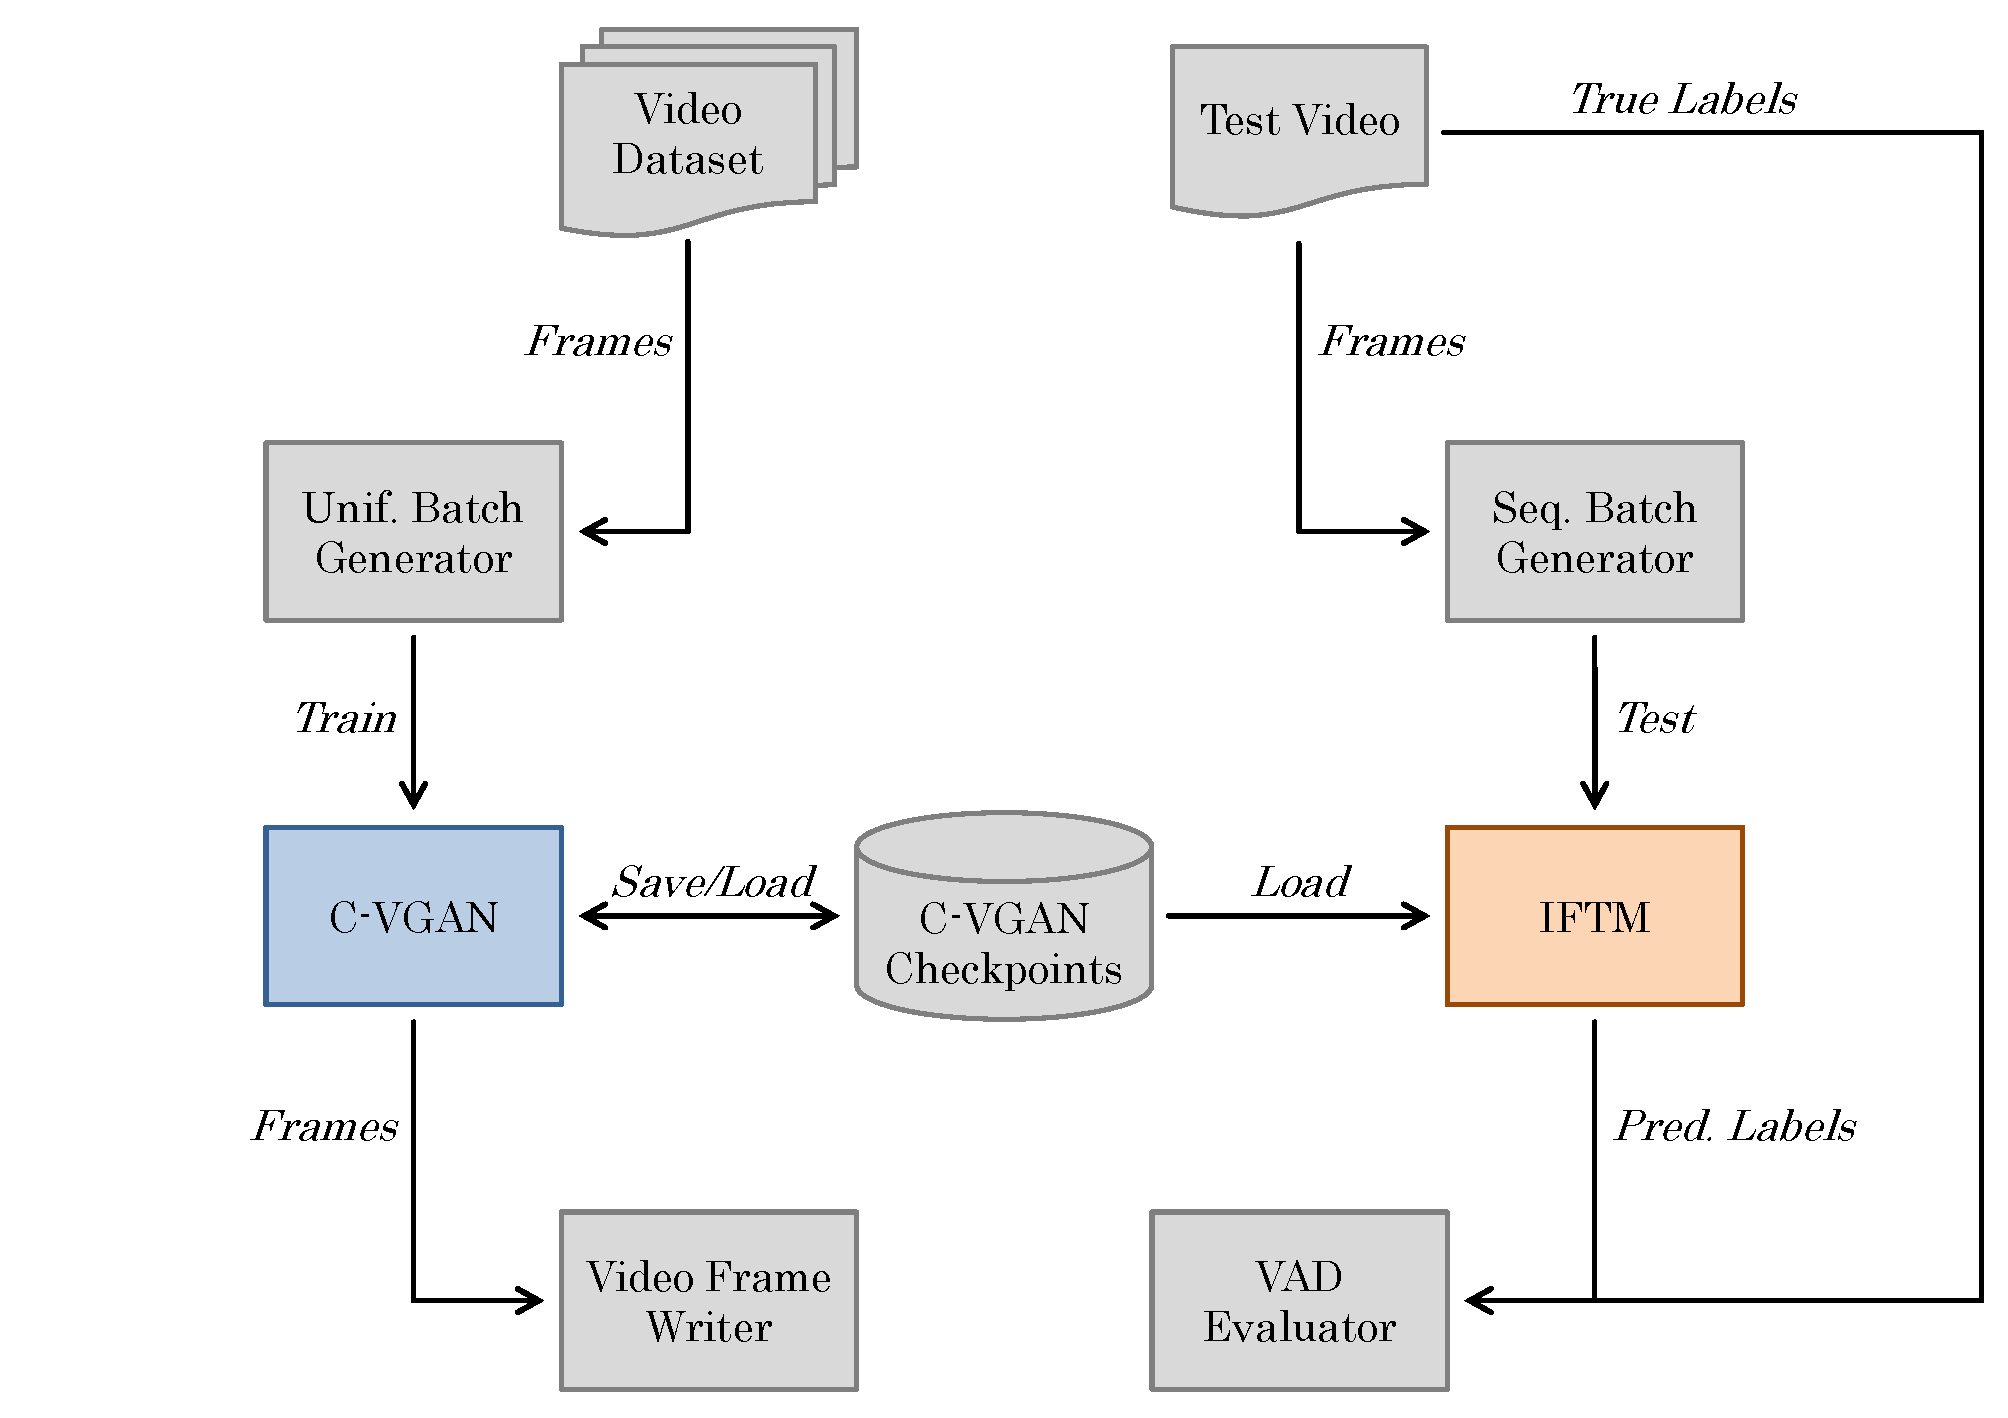
\includegraphics[width=1\textwidth]{graphics/anomalyDetection/ads/system/system.pdf}
  \caption[Components of the video anomaly detection system.]{Components of the video anomaly detection system.}
  \label{fig:ads_overview}
\end{figure}

Putting the different parts of our anomaly detection system (ADS) together, in this section we present an overview of the system depicted in Figure \ref{fig:ads_overview} and go into more detail how we further process the videos that were created and preprocessed as described in the preceding section. Due to the use of a video generation model, the videos have to be first read in a certain way to allow training with the video frames available. We present two batch generators, one to be used during training and a sequential one for evaluation purposes. Afterwards, we explain how the adapted C-VGAN for next-frame prediction is trained and how a trained generator model is loaded and integrated into IFTM at runtime. This includes an overview of the hyperparameters that have to be set. Finally for the last step, we give a brief introduction how the results of both C-VGAN and IFTM are visualized and postprocessed for evaluation.


% Sample and Batch Generation
\subsection{Sample and Batch Generation} \label{subsec:batch_generation}

During training and video generation using the adapted C-VGAN models, the generator and discriminator model only accept 8 frame long videos per sample (a single video clip that is generated or discriminated), and 7 frame long video clips as spatio-temporal input for the next-frame forecasting generator model. So one has to create thousands of smaller video clips from a single video file that can be read in efficient manner. Vondrick et al. during the evaluation of VGAN which requires 32 frames per video clip encountered the same challenge and solved it by concatenating the decoded raw frames of a 32 frame long video clip vertically and saving the resulting file as an image \cite{vondrick2016generating}. Reading these input files requires additional array transformations to transform the 2-dimensional data into a 3-dimensional one, but at the same time it saves additional IO and decoding operations. However, in our use-case, this kind of preprocessing would be redundant: Samples in our case overlap, because the model always has to predict the next frame of the stream and that stream during the detection phase is processed one frame to the next. Meanwhile in the VGAN evaluation by Vondrick et al., the different video clips that were used for training and evaluation were independent from each other. For our data set, the required redundancies to create one image file per video clip would explode the size of the available storage. But even fulfilling the minimum requirement when pre-decoding all videos, i.e. storing every video frame, each decoded as an raw image on a disk is not feasible. It would result in half a gigabyte for $18,000$ frames or one hour of video material, while there are 240 files to be decoded. Furthermore the increase in IO operations would result in a bottleneck, because the frames have to be load from disk individually, every time a sample is generated.

This challenge requires an efficient online decoding of video frames during training of C-VGAN and the anomaly detection phase of IFTM. The video files that are MP4 compressed are loaded into the memory at the start of training and evaluation, but frames and thus samples have to be decoded and created on the fly. Using the OpenCV\footnote{\url{https://opencv.org}} library, one can decode a video frame by frame: Each decoding-call will return a 2-dimensional byte array with three color channels in BGR order. The order of the color channels can be kept this way as it will used for the all training and detection phases and our models do not have a channel order preference. Another challenge exists however in the form of the byte array, which is unuseable by a neural network that works with 32-bit floats. After the necessary type conversion of the entire 2D-array, all pixel color values $x$, which are in the range of $[0, 255]$ are also normalized to a range of $[-1, 1]$ with the following equation:

\begin{equation} \label{eq:norm}
N(x) = \frac{x - 127.5}{127.5}
\end{equation}

\begin{figure}
  \centering
	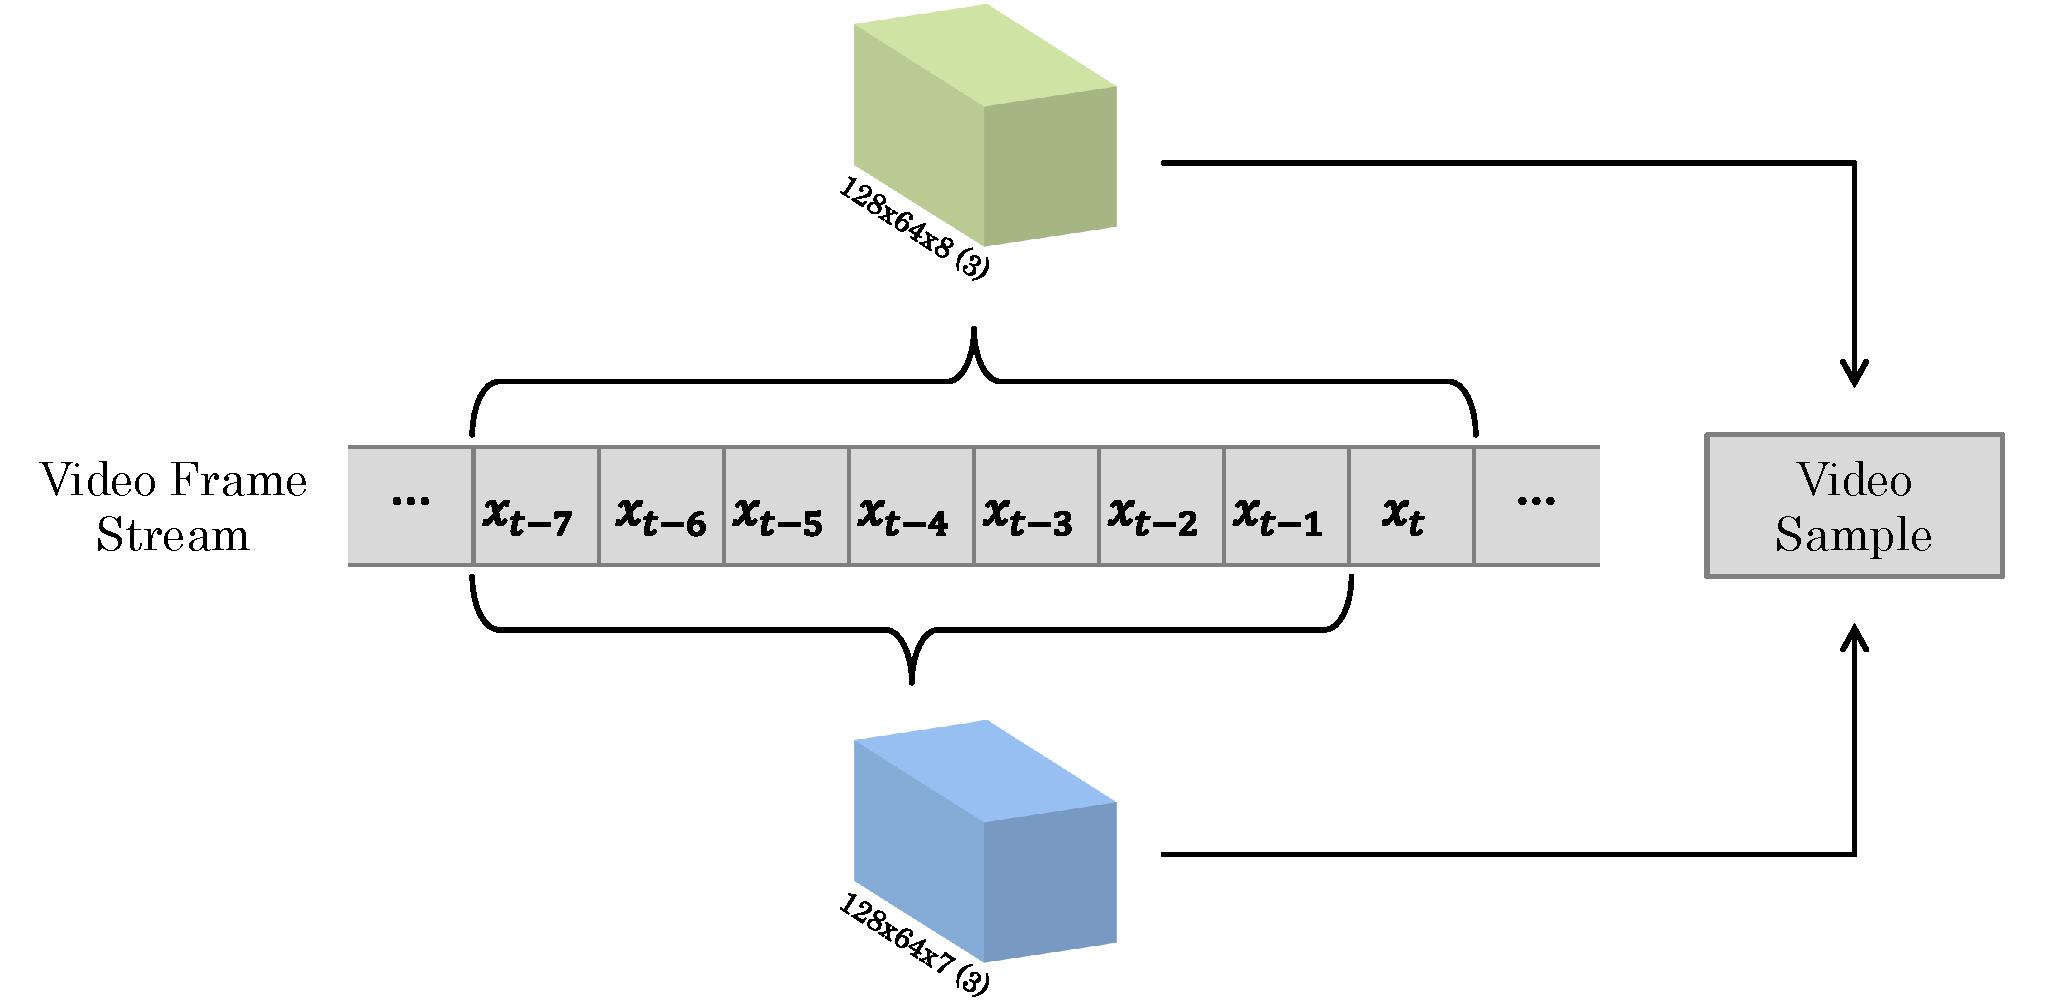
\includegraphics[width=1\textwidth]{graphics/anomalyDetection/ads/sampleGeneration/sampleGeneration.pdf}
  \caption[Creation of a video sample from a frame stream.]{Creation of a video sample from a frame stream, consisting of two video clips arranged as space-time cuboids. The green one serves as input for C-VGAN discriminator, while the blue cuboid will be passed to the generator to perform next-frame prediction.}
  \label{fig:sample_generator}
\end{figure}

This kind of scaling, also used for general DCGANs but also VGAN and C-VGAN, helps with the convergence speed, matching the range of the hyperbolic tangent activation function used in the final layer(s) of the generator \cite{radford2015unsupervised}. Thus, reading a video's frame into arrays, then converting and scaling them, can be used $8$ times to extract the required number of consecutive frames, as shown in Figure \ref{fig:sample_generator}: Stacking the frames as a 3-dimensional cube, this object is duplicated and the last frame is sliced off. The resulting object, a $7$ frame long video clip without its last observation serves as the video input for the next-frame prediction model, while the other one represents the discriminator input. These two together represent a single sample that is passed to the adapted C-VGAN model during training.

Data preprocessing is not done yet, as passing singular samples to the GANs is not the intention during training or testing. GANs are trained by taking a number of samples from the entire training set and passing them to the model as a mini-batch. This is repeated until a percentage of the training data set --- ideally the entire data set,  was passed to the model and this so called epoch is repeated multiple times until a convergence or some other stopping criterion is reached (see Section \ref{sec:gans}). Due to the way the models train and how the inputs are passed and processed by the models, it is important that these mini-batches are ideally sampled independently from the structure of the data. Else a model might learn the structure of the batches during a training step and adapt to it, while being unable to generalize well during testing \cite{bengio2012practical}. Or worse, because during the first batches in an epoch, the model first learns using one type of features witnessed in the batches, before in the second half of the training epoch, it sees the another type. For example, when the video data of a single day is sequentially transformed into batches and then passed to the model, the first batches exclusively contain batches during the day, before only batches with video clips from the night time are witnessed by the models. To improve the quality of the model, some form of randomness for the sample and batch generation is required. First, the overall order of the batches can be shuffled, but for the internal structure of the individual mini-batches, one has to adjust the kind of sampling that is done. Random sampling to create a batch is not only very inefficient but it risks collisions, i.e. sampling the same video clips multiple times during a training epoch, which is also not desired.

As this issue is only relevant during the training phase, because during detection the order of the samples and thus the batches should be treated as a time series, we propose two different batch generators to be used in the two phases respectively. Both of these create samples with the same mentioned structure and the same preprocessing (type conversion and scaling), but the order and structure of the batches and the samples within them differs. The rest of this section will present these and how the two are utilized in our framework shown in Figure \ref{fig:ads_overview}.

\paragraph{Uniform Batch Generator} \label{par:uniform_bgen}
The first of the two batch generators is used during the training phase of the GANs. It attempts to sample the data set in some form of uniform fashion, loading the individual batches of samples in non-sequential order. This has to be done in deterministic and stateless manner, because batch generation will be done concurrently. Else the batch generator is unable to keep up with the training coordinator process of the models. Thus, when loading the videos of the training data set into memory, they are structured as follows: As the number of days is assumed to be fixed but arbitrary, each day is organized as an individual structure. Then, each day is split into six disjunctive subsets of files, therefore four different hours of the day, as shown on the upper half of Figure \ref{fig:uniform_bgen}. This way, when sampling video clips from these disjunctive sets, one gets video clips during both the night and the day when drawing samples from the four respective hours of files uniformly.

To ensure the deterministic and stateless nature, we utilize the id of a batch $b_i$ and map it to a day $d$ and to one of its disjunctive subsets $s$ using Equation \ref{eq:day} and \ref{eq:subset}. Assuming an equal number of to be generated batches per day --- the number not only depends on the sample size (in our case 8 frames), but also on the batch size that is a hyperparameter explained in the next section, one can sample a quarter of a batch from each of the four videos of the disjunctive subset $s$. When doing so, sampling is done in sequential manner starting from an offset $t$ in each of the four videos, as depicted in Equation \ref{eq:offset}. All frames that came before that point were already used by lower batch ids to create samples from. Starting decoding from an offset on an already opened video file can be done using OpenCV. Note that in case of this batch generator, samples in itself are also disjunctive and their frames do not overlap. Because the selection of day, subset, and offset is done based on $b_i$ and the ids are shuffled at the beginning of every epoch, only the order of the batches changes while the internal structure of each $b_i$ remains constant.

\begin{figure}
	\centering
	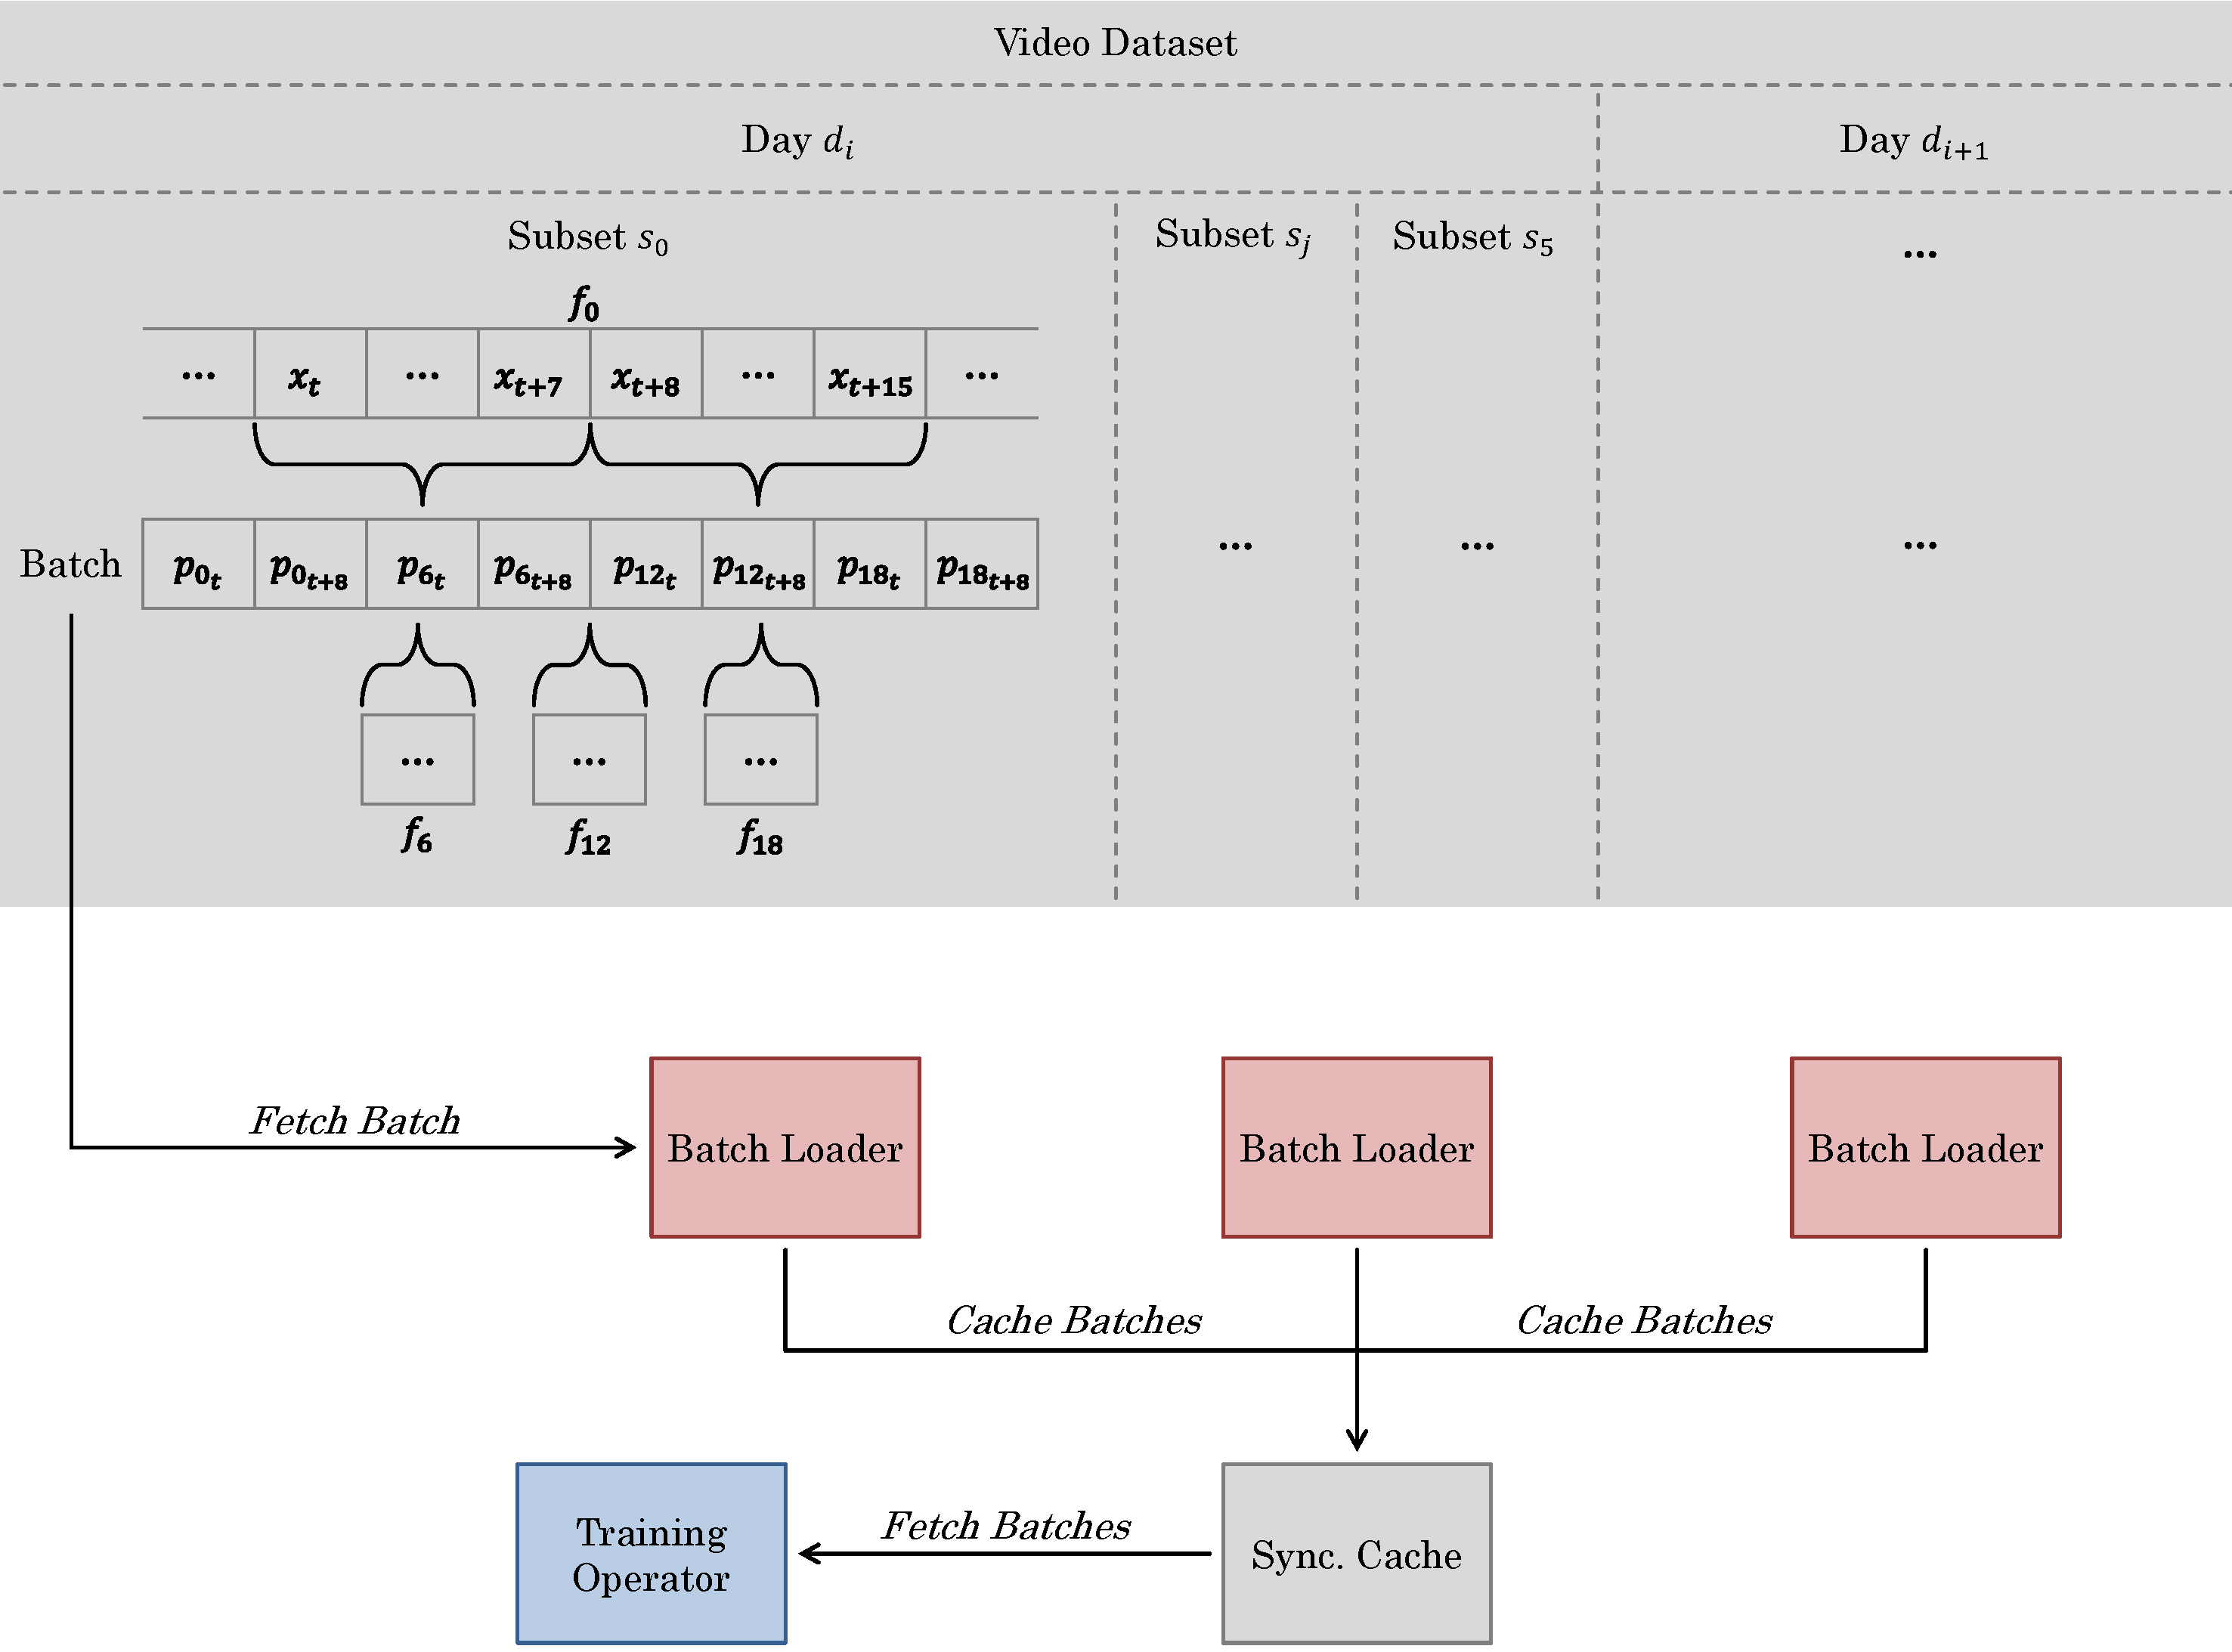
\includegraphics[width=1\textwidth]{graphics/anomalyDetection/ads/batchGeneration/uniform/uniformBatchGenerator.pdf}
  \caption[Creation of a batch sampling from different hours of a day.]{Generation of a batch uniformly sampling from four different files (\textit{f}) of a day, with each file containing one hour of video material. These hours are grouped together in disjunctive subsets (\textit{s}), of which six exist per day (\textit{d}). Batches are fetched from the generator and then cached concurrently by multiple loaders. The operator that handles the training can then fetch ready batches to pass them to the models.}
  \label{fig:uniform_bgen}
\end{figure}

\begin{equation} \label{eq:day}
d = \left \lfloor {\frac{b_i}{batchesPerDay}} \right \rfloor
\end{equation}

\begin{equation} \label{eq:subset}
s = \left \lfloor {\frac{b_i \text{ mod } batchesPerDay}{quarterBatchesPerHour}} \right \rfloor
\end{equation}

\begin{equation} \label{eq:offset}
t = framesPerQuarterBatch \cdot (b_i  \text{ mod } batchesPerDay  \text{ mod } quarterBatchesPerHour)
\end{equation}

As the loading of batches from the batch generator is done concurrently, the access to any video has to be mutual exclusive at any point at runtime. Each of the batch loaders get a shuffled subset of $b_i$ with $i \in [0,N-1]$ with $N$ being the total number of batches that need to be generated. This process is depicted in Figure \ref{fig:uniform_bgen}. Generated batches are passed from the workers to a synchronized cache, from which the operator that coordinates the training of the models draws batches from. This reduces idle times for the training process as the workers in the background provide a constant stream of batches to it. The number of workers and the size of the synchronized cache can be tuned, but they depend on the hardware available and have no influence on the actual quality of the final trained model. During our evaluation, we used $4$ workers to load batches into the synchronized cache that was of size $c = \left \lfloor {\frac{2048}{batchSize}} \right \rfloor$. This cache size proved to be sufficient enough in removing any idle times during training, i.e. the bottleneck was not the fetching of the dataset, but the actual training procedure itself.

\paragraph{Sequential Batch Generator} \label{par:sequential_bgen}

While the generated batches in the training phase can be sampled in any way imaginable, because the adapted C-VGAN model makes predictions for a sample independent from other inputs besides the 7 frames passed to it for a prediction, the detection phase is different: As was explained in Section \ref{sec:vad}, IFTM, as modified to our use case, makes forecasting, computation of the prediction error, and the mapping to the binary label (anomaly or not) online, treating the video data as a stream. Although this is doable in real time, it is not desired during evaluation: Because the C-VGAN models are deployed on a GPU as explained in the following section, one can make use of all the video memory and processing units available and parallelize this part of the evaluation system as well for major speedups \cite{owens2008gpu, abadi2016tensorflow}. But running several next-frame predictions for a multitude of samples at the same step in parallel, implies that some form of batch generation is required again. 

To keep the samples in order of their occurrence in the stream, samples are aggregated into batches following Figure \ref{fig:sequential_bgen}: This time, files are structured as a list from which samples are generated from, one file after another. For each file, samples are created by sliding a window with size $8$ with step size $1$ over the frames and this is done until the required number of samples for a batch have been created. Same as the other batch generator this process can be done deterministically and statelessly, by mapping batch id $b_i$ again to a file ($f$), illustrated in Equation \ref{eq:day2}, before reading samples starting from position $t$ of the selected video file. This again assumes videos of equal length and thus number of frames.

\begin{figure}
	\centering
	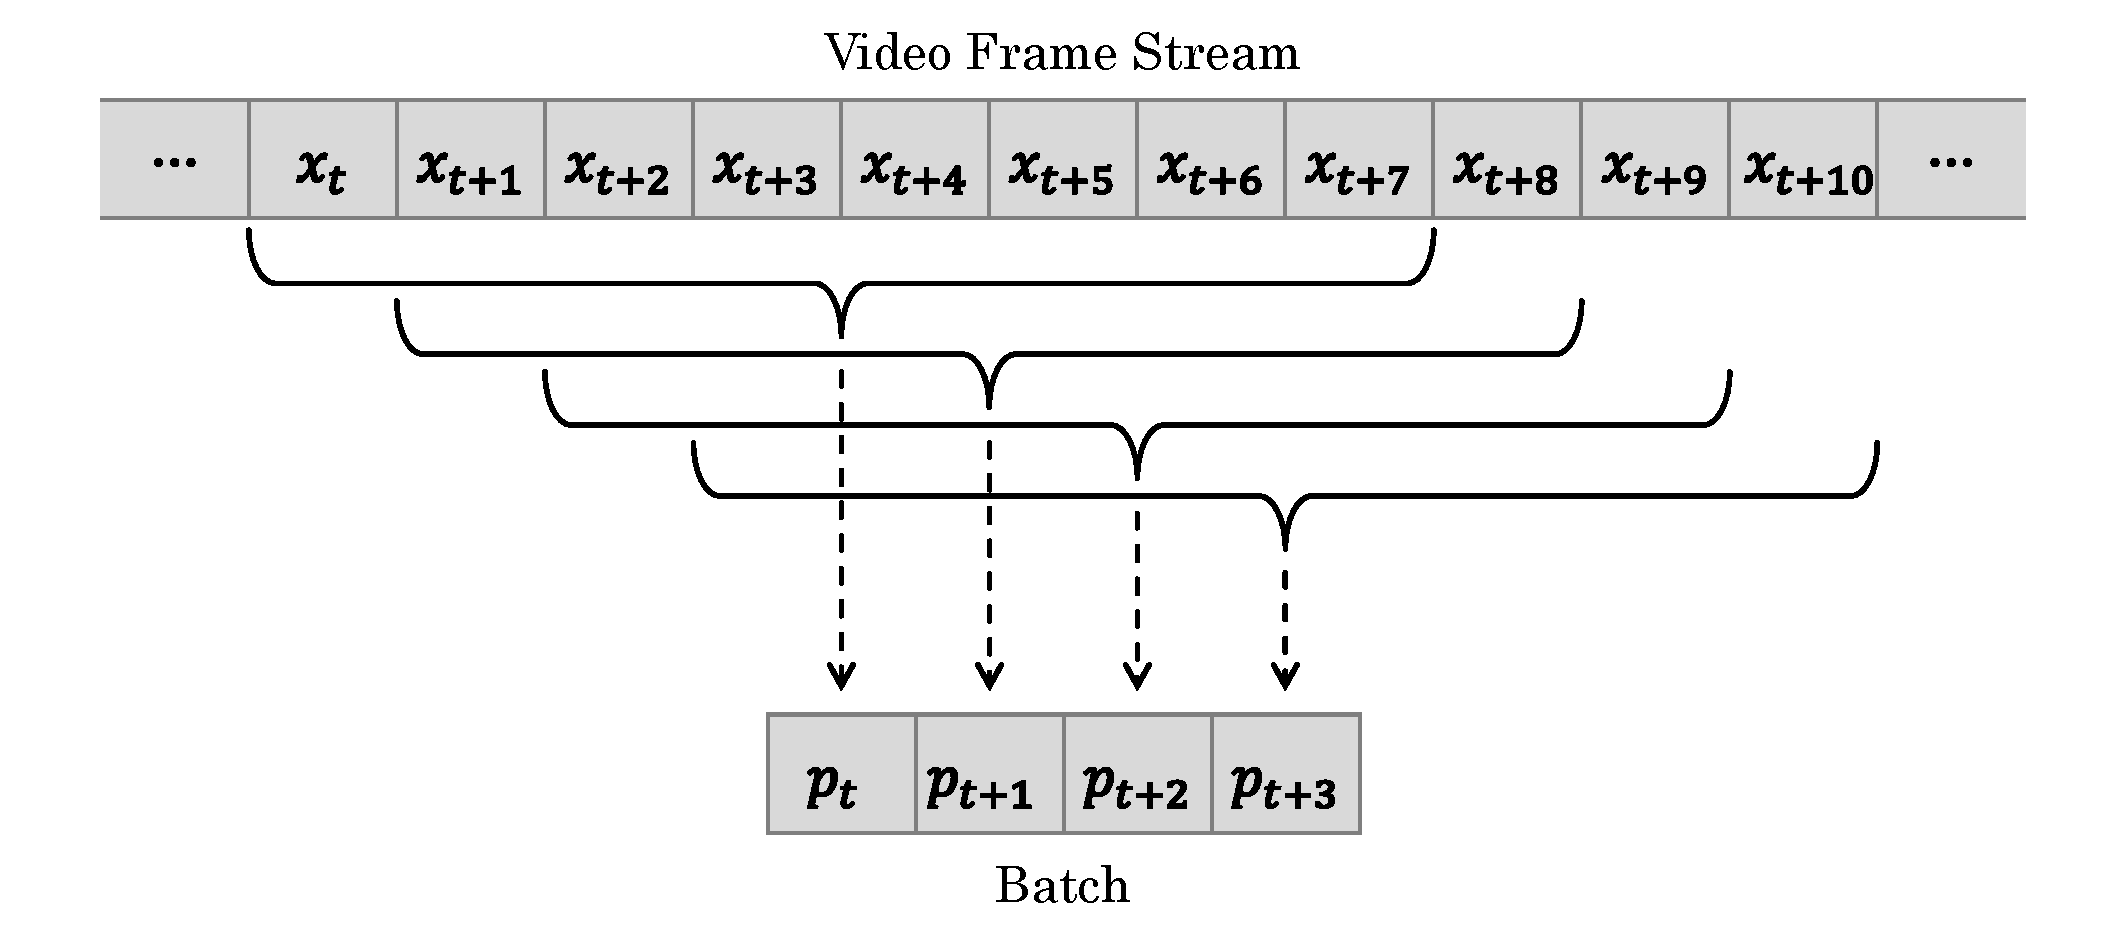
\includegraphics[width=1\textwidth]{graphics/anomalyDetection/ads/batchGeneration/sequential/sequentialBatchGenerator.pdf}
  \caption[Creation of a batch that consists of consecutive samples.]{Creation of a batch that consists of four consecutive and overlapping samples, using a sliding window to aggregate frames into samples (\textit{p}), and samples into batches.}
  \label{fig:sequential_bgen}
\end{figure}

\begin{equation} \label{eq:day2}
f = \left \lfloor {\frac{b_i}{batchesPerFile}} \right \rfloor
\end{equation}

\begin{equation} \label{eq:offset2}
t = framesPerBatch \cdot (b_i  \text{ mod } batchesPerFile)
\end{equation}

Although one could now use this sequential batch generator with multiple workers to fetch data faster, it is not advised due to the inherent order of a stream: Unlike in the other generator, batches can not be read out of order, nor can they be placed in the synchronized cache in an arbitrary one, because the samples in every batch have to be matched to their true labels for evaluation. This requires some overhead to synchronize the write order for multiple batch loaders. Meanwhile in our data set presented in Section \ref{sec:dataset}, there is only one video file that has to be read in that manner, which makes such a speedup not only unnecessary, but also impossible. As already mentioned above, access to a video is mutual exclusive, so different batch loaders would only alternate their access to that single video file between each other. Compared to the $240$ video files of the training set, reading the much smaller evaluation set can be done in this evaluation framework with a single worker, creating batches in order. It is to note however that the batch size has no influence on the results during prediction and thus can be as great as the video memory permits, providing some additional speedup. 


% C-VGAN Training, Model Creation
\subsection{C-VGAN Adaption} \label{subsec:framework_cvgan}

\begin{table}
	\centering
	\begin{tabular}{ | l | p{9cm} | r |}
	\toprule
	\textbf{Hyperparameter} & \textbf{Description} & \textbf{Default Value} \\
	\midrule
  $\lambda$ & Weight of the reconstruction loss term for the first 7 frames of the generator output. Limits the degrees of freedom, i.e. how much past frames determine the forecasting. & $10$ \\ \hline
  $cf$ & Number of convolutional filters (channels) in the first layer of the discriminator. The value is doubled for each consecutive step of the CNN stack. Greater values empower the model, while smaller ones impair it.  & $32$ \\ \hline
  $dr$ & Dropout rate at which input units after every convolutional layer in the discriminator get randomly set to 0 during training. Regularization parameter. & $0.0$ \\ \hline
  $bs$ & Batch size; number of samples that are passed to the models at each training step. & $64$ \\ \hline
  $lr$ & Learning rate; step size of optimizers during training. & $0.002$ \\
	\bottomrule
	\end{tabular}
	\caption[Hyperparameters of the modified C-VGAN next-frame prediction model.]{Summary of the non-fixed hyperparameters of the modified C-VGAN next-frame prediction model.}
	\label{tab:cvgan_params}
\end{table}

For building our proposed adapted architecture for next-frame prediction, we take the two models presented in Section \ref{subsec:vgan_mod_2} and define them using TensorFlow. TensorFlow, as the name suggests, uses dataflow graphs to represent computations and the operations that mutate the states in it \cite{abadi2016tensorflow}. Because our model consists of two components --- a generator and a discriminator, that have to be trained in adversarial fashion, we define the two models using the functional API by Keras that serves as an abstraction layer ontop of TensorFlow \cite{chollet2015keras}. For the training procedure, we define a custom training loop. At each step during training, the current batch is passed to the discriminator and the generator, with the latter one using the first 7 frames of the sample as input. Losses are computed using the adapted value function of C-VGAN for next-frame prediction. For optimization of the models the Adam optimizer \cite{kingma2014adam} was chosen; one for the discriminator and another for the generator model. In VGAN and C-VGAN, Vondrick et al. use Adam with a learning rate of $0.002$ and a momentum term of $\beta = 0.5$, while using a batch size of $64$. For training models the batch size serves as a hyperparameter, because the value function is computed over the entire batch, i.e. the losses for each sample in the batch are computed and then summed up. This however can bring additional hurdles, if the batch size is large, but the data set is diverse \cite{radiuk2017impact}: Meaningful observations in the batch might get discarded and ignored, because the total loss for a batch is driven by the majority. And with the model being tuned through the minimization of the loss for each batch, rare but normal observations will not find their representation within the model. But at the same time a large batch size also helps with suppressing anomalous observations that might be encountered in the training data set. Although Adam is an adapted optimizer, its learning rate might need adjustment when tuning the batch size \cite{krizhevsky2014one}. To keep the variance of the gradient expectation constant, the learning rate is multiplied by the square root of $k$, with $k$ being the factor by which the batch size was increased. The momentum was chosen to stay fixed and mirrors the original configuration of DCGAN and VGAN.

The other hyperparameters for both generator and discriminator, that were already explained in detail in Section \ref{subsec:vgan_mod_2}, also have to be set. Their default values are also included in Table \ref{tab:cvgan_params}. When setting these hyperparameters and training the configured model, training has to be done for several epochs over the training set. Because training takes up to $2$ days of computations (see the next chapter), intermediate results of the models are stored to disk after every $N$ epochs, with the hyperparameter configuration attached. This not only serves as fault tolerance, but also a means to evaluate different configurations in quick succession by simply loading and evaluating one after the other. In addition, one can load and evaluate a model from different points in training, to see whether the quality of the model has degraded over the epochs; see Section \ref{par:failure_modes} for details regarding collapse in training and early stopping.

For the evaluation in the next chapter in Section \ref{sec:cvgan_eval}, the losses per batch are averaged and logged for each epoch during training. Moreover, after each epoch one can also validate the quality of the current models with a separate validation data set and the average batch loss is then also logged.


% IFTM Training, Predicting
\subsection{IFTM Adaption} \label{subsec:framework_iftm}

To load offline trained models into the adapted version of IFTM from Section \ref{sec:vad} to perform VAD, one has to select one of the stored generator models from the preceding section. Loading it via the TensorFlow checkpoint API\footnote{\url{www.tensorflow.org/guide/checkpoint}}, that forecasting model is then defined as the IF of the IFTM anomaly detection model. Afterwards, as explained in the adaptation of IFTM, all training samples used during the training of the generator model have to be passed to the model again to compute the prediction error for their respective 8th frame. Aggregating the distribution of the errors into its mean and standard deviation, one can now compute the (static) threshold value for the IFTM. There are no additional hyperparameters for this version of IFTM beside the ones for the underlying next-frame forecasting model, which do not change after loading the checkpoint.

As this procedure concludes the offline training phase, the detection phase begins: Using the sequential batch generator, batches of samples are passed to the IF to perform next-frame prediction. Afterwards the prediction error and the mapping to the binary label, 0=normal and 1=anomalous, is done for each sample in the batch. For evaluation purposes, the error value and the binary prediction for each sample are logged as a tuple. Based on the former metric, we will also analyze in the next chapter how IFTM using video generation forecasting models performs on our evaluation data set.


% Evaluation and Visualization
\subsection{Postprocessing} \label{subsec:postprocessing}

When postprocessing the generated video samples of C-VGAN, forecast frames for the evaluation data set are written to disk as PNG images for visual evaluation, i.e. how realistic these predictions actually are. Doing so, the data type is also reversed to 8-bit format and a scaling of each pixel color value of $[0,255]$. In addition, during training, a fixed set of input samples are passed to the forecasting model to run a prediction on after every epoch. These predictions are also written to disk as animated GIFs to monitor the quality of the generated videos. In Section \ref{subsec:cvgan_eval_method} of the next chapter, an in-depth overview of the evaluation methods for the next-frame prediction model is provided.

For the evaluation of the VAD system using IFTM, its binary predictions for each sample are compared to the ground truth, as the true label of each frame in the evaluation data set is available in a separate CSV file. The results of thereof are aggregated into a confusion matrix, which can then be utilized to compute several metrics to measure the quality of the model. In the following chapter in Section \ref{subsec:vad_eval_method} we will show our chosen evaluation metrics for IFTM, and how they are inferred from the matrix, before we present and discuss our results for different configurations of the underlying models. 